\documentclass[twoside]{book}

% Packages required by doxygen
\usepackage{calc}
\usepackage{doxygen}
\usepackage{graphicx}
\usepackage[utf8]{inputenc}
\usepackage{makeidx}
\usepackage{multicol}
\usepackage{multirow}
\usepackage{textcomp}
\usepackage[table]{xcolor}

% Font selection
\usepackage[T1]{fontenc}
\usepackage{mathptmx}
\usepackage[scaled=.90]{helvet}
\usepackage{courier}
\usepackage{amssymb}
\usepackage{sectsty}
\renewcommand{\familydefault}{\sfdefault}
\allsectionsfont{%
  \fontseries{bc}\selectfont%
  \color{darkgray}%
}
\renewcommand{\DoxyLabelFont}{%
  \fontseries{bc}\selectfont%
  \color{darkgray}%
}

% Page & text layout
\usepackage{geometry}
\geometry{%
  a4paper,%
  top=2.5cm,%
  bottom=2.5cm,%
  left=2.5cm,%
  right=2.5cm%
}
\tolerance=750
\hfuzz=15pt
\hbadness=750
\setlength{\emergencystretch}{15pt}
\setlength{\parindent}{0cm}
\setlength{\parskip}{0.2cm}
\makeatletter
\renewcommand{\paragraph}{%
  \@startsection{paragraph}{4}{0ex}{-1.0ex}{1.0ex}{%
    \normalfont\normalsize\bfseries\SS@parafont%
  }%
}
\renewcommand{\subparagraph}{%
  \@startsection{subparagraph}{5}{0ex}{-1.0ex}{1.0ex}{%
    \normalfont\normalsize\bfseries\SS@subparafont%
  }%
}
\makeatother

% Headers & footers
\usepackage{fancyhdr}
\pagestyle{fancyplain}
\fancyhead[LE]{\fancyplain{}{\bfseries\thepage}}
\fancyhead[CE]{\fancyplain{}{}}
\fancyhead[RE]{\fancyplain{}{\bfseries\leftmark}}
\fancyhead[LO]{\fancyplain{}{\bfseries\rightmark}}
\fancyhead[CO]{\fancyplain{}{}}
\fancyhead[RO]{\fancyplain{}{\bfseries\thepage}}
\fancyfoot[LE]{\fancyplain{}{}}
\fancyfoot[CE]{\fancyplain{}{}}
\fancyfoot[RE]{\fancyplain{}{\bfseries\scriptsize Generated on Sun Mar 12 2017 01\-:38\-:35 for Path Finding Project by Doxygen }}
\fancyfoot[LO]{\fancyplain{}{\bfseries\scriptsize Generated on Sun Mar 12 2017 01\-:38\-:35 for Path Finding Project by Doxygen }}
\fancyfoot[CO]{\fancyplain{}{}}
\fancyfoot[RO]{\fancyplain{}{}}
\renewcommand{\footrulewidth}{0.4pt}
\renewcommand{\chaptermark}[1]{%
  \markboth{#1}{}%
}
\renewcommand{\sectionmark}[1]{%
  \markright{\thesection\ #1}%
}

% Indices & bibliography
\usepackage{natbib}
\usepackage[titles]{tocloft}
\setcounter{tocdepth}{3}
\setcounter{secnumdepth}{5}
\makeindex

% Hyperlinks (required, but should be loaded last)
\usepackage{ifpdf}
\ifpdf
  \usepackage[pdftex,pagebackref=true]{hyperref}
\else
  \usepackage[ps2pdf,pagebackref=true]{hyperref}
\fi
\hypersetup{%
  colorlinks=true,%
  linkcolor=blue,%
  citecolor=blue,%
  unicode%
}

% Custom commands
\newcommand{\clearemptydoublepage}{%
  \newpage{\pagestyle{empty}\cleardoublepage}%
}


%===== C O N T E N T S =====

\begin{document}

% Titlepage & ToC
\hypersetup{pageanchor=false}
\pagenumbering{roman}
\begin{titlepage}
\vspace*{7cm}
\begin{center}%
{\Large Path Finding Project \\[1ex]\large 1.\-0 }\\
\vspace*{1cm}
{\large Generated by Doxygen 1.8.6}\\
\vspace*{0.5cm}
{\small Sun Mar 12 2017 01:38:35}\\
\end{center}
\end{titlepage}
\clearemptydoublepage
\tableofcontents
\clearemptydoublepage
\pagenumbering{arabic}
\hypersetup{pageanchor=true}

%--- Begin generated contents ---
\chapter{Hierarchical Index}
\section{Class Hierarchy}
This inheritance list is sorted roughly, but not completely, alphabetically\-:\begin{DoxyCompactList}
\item \contentsline{section}{Edge}{\pageref{d8/d8c/classEdge}}{}
\item \contentsline{section}{Map}{\pageref{d7/db0/classMap}}{}
\item \contentsline{section}{Node}{\pageref{df/dd0/classNode}}{}
\item \contentsline{section}{Path\-Finding\-Algorithm}{\pageref{d7/df1/classPathFindingAlgorithm}}{}
\begin{DoxyCompactList}
\item \contentsline{section}{A\-Star\-Algorithm}{\pageref{d5/d12/classAStarAlgorithm}}{}
\end{DoxyCompactList}
\end{DoxyCompactList}

\chapter{Class Index}
\section{Class List}
Here are the classes, structs, unions and interfaces with brief descriptions\-:\begin{DoxyCompactList}
\item\contentsline{section}{\hyperlink{classAStarAlgorithm}{A\-Star\-Algorithm} \\*Class definition of \hyperlink{classAStarAlgorithm}{A\-Star\-Algorithm} class which is derived from base class \hyperlink{classPathFindingAlgorithm}{Path\-Finding\-Algorithm} for path planning }{\pageref{d5/d12/classAStarAlgorithm}}{}
\item\contentsline{section}{\hyperlink{classEdge}{Edge} \\*Class that maintains edge cost between two nodes in a map }{\pageref{d8/d8c/classEdge}}{}
\item\contentsline{section}{\hyperlink{classMap}{Map} \\*Class definition of \hyperlink{classMap}{Map} used for keeping map information for path planning }{\pageref{d7/db0/classMap}}{}
\item\contentsline{section}{\hyperlink{classNode}{Node} \\*Class that maintains node information in a map }{\pageref{df/dd0/classNode}}{}
\item\contentsline{section}{\hyperlink{classPathFindingAlgorithm}{Path\-Finding\-Algorithm} \\*Class that implements the basic functions reqiured for path finding algorithm }{\pageref{d7/df1/classPathFindingAlgorithm}}{}
\end{DoxyCompactList}

\chapter{File Index}
\section{File List}
Here is a list of all files with brief descriptions\-:\begin{DoxyCompactList}
\item\contentsline{section}{app/\hyperlink{AStarAlgorithm_8cpp}{A\-Star\-Algorithm.\-cpp} \\*Implementation of class \hyperlink{classAStarAlgorithm}{A\-Star\-Algorithm} methods }{\pageref{d5/d0e/AStarAlgorithm_8cpp}}{}
\item\contentsline{section}{app/\hyperlink{app_2main_8cpp}{main.\-cpp} }{\pageref{d5/d9c/app_2main_8cpp}}{}
\item\contentsline{section}{app/\hyperlink{Map_8cpp}{Map.\-cpp} \\*Implementation of class \hyperlink{classMap}{Map} and its methods to maintain map info of a path finding algorithm }{\pageref{d3/d92/Map_8cpp}}{}
\item\contentsline{section}{app/\hyperlink{PathFindAlgorithm_8cpp}{Path\-Find\-Algorithm.\-cpp} \\*Implementation of class Path\-Find\-Algorithm methods }{\pageref{d2/d4f/PathFindAlgorithm_8cpp}}{}
\item\contentsline{section}{include/\hyperlink{AStarAlgorithm_8hpp}{A\-Star\-Algorithm.\-hpp} \\*Definition of class \hyperlink{classAStarAlgorithm}{A\-Star\-Algorithm} }{\pageref{d8/d4b/AStarAlgorithm_8hpp}}{}
\item\contentsline{section}{include/\hyperlink{Edge_8hpp}{Edge.\-hpp} \\*Definition of class \hyperlink{classEdge}{Edge} }{\pageref{dc/d91/Edge_8hpp}}{}
\item\contentsline{section}{include/\hyperlink{Map_8hpp}{Map.\-hpp} \\*Definition of class \hyperlink{classMap}{Map} }{\pageref{dc/dbe/Map_8hpp}}{}
\item\contentsline{section}{include/\hyperlink{Node_8hpp}{Node.\-hpp} \\*Definition of class \hyperlink{classNode}{Node} }{\pageref{d7/dc6/Node_8hpp}}{}
\item\contentsline{section}{include/\hyperlink{PathFindAlgorithm_8hpp}{Path\-Find\-Algorithm.\-hpp} \\*Definition of class Path\-Find\-Algorithm }{\pageref{de/dbc/PathFindAlgorithm_8hpp}}{}
\item\contentsline{section}{test/\hyperlink{test_2main_8cpp}{main.\-cpp} }{\pageref{d4/d15/test_2main_8cpp}}{}
\item\contentsline{section}{test/\hyperlink{test_8cpp}{test.\-cpp} \\*Implementation of unit test for \hyperlink{classAStarAlgorithm}{A\-Star\-Algorithm} }{\pageref{df/dac/test_8cpp}}{}
\end{DoxyCompactList}

\chapter{Class Documentation}
\hypertarget{classAStarAlgorithm}{\section{A\-Star\-Algorithm Class Reference}
\label{classAStarAlgorithm}\index{A\-Star\-Algorithm@{A\-Star\-Algorithm}}
}


Class definition of \hyperlink{classAStarAlgorithm}{A\-Star\-Algorithm} class which is derived from base class \hyperlink{classPathFindingAlgorithm}{Path\-Finding\-Algorithm} for path planning.  




{\ttfamily \#include $<$A\-Star\-Algorithm.\-hpp$>$}

Inheritance diagram for A\-Star\-Algorithm\-:\begin{figure}[H]
\begin{center}
\leavevmode
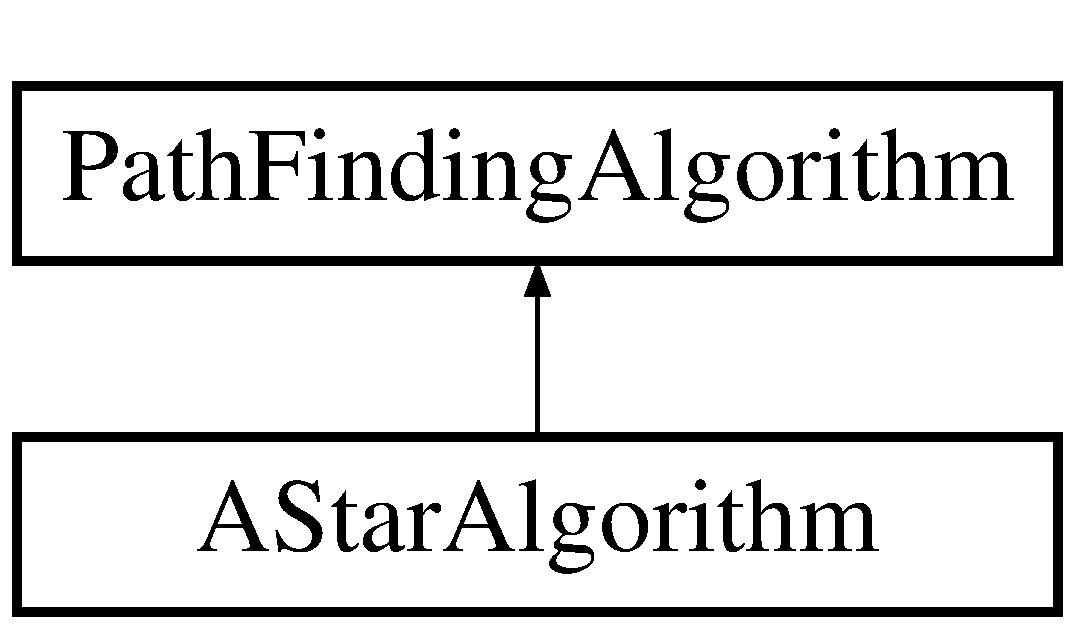
\includegraphics[height=2.000000cm]{d5/d12/classAStarAlgorithm}
\end{center}
\end{figure}
\subsection*{Public Member Functions}
\begin{DoxyCompactItemize}
\item 
\hyperlink{classAStarAlgorithm_afa80dc5f04400d38c43a609da0ce948e}{A\-Star\-Algorithm} ()
\begin{DoxyCompactList}\small\item\em Constructor of \hyperlink{classAStarAlgorithm}{A\-Star\-Algorithm} class. \end{DoxyCompactList}\item 
\hyperlink{classAStarAlgorithm_a2ab75ee9abadf5919c22fe1ee812b8d4}{$\sim$\-A\-Star\-Algorithm} ()
\begin{DoxyCompactList}\small\item\em Deconstructor of \hyperlink{classAStarAlgorithm}{A\-Star\-Algorithm} class. \end{DoxyCompactList}\item 
bool \hyperlink{classAStarAlgorithm_af3adf65228c56523489d3bd4e278e66f}{comput\-Path} (double)
\begin{DoxyCompactList}\small\item\em Compute shortest path using given start, goal nodes indices, and weight for heuristic estimates. \end{DoxyCompactList}\end{DoxyCompactItemize}
\subsection*{Additional Inherited Members}


\subsection{Detailed Description}
Class definition of \hyperlink{classAStarAlgorithm}{A\-Star\-Algorithm} class which is derived from base class \hyperlink{classPathFindingAlgorithm}{Path\-Finding\-Algorithm} for path planning. 

\subsection{Constructor \& Destructor Documentation}
\hypertarget{classAStarAlgorithm_afa80dc5f04400d38c43a609da0ce948e}{\index{A\-Star\-Algorithm@{A\-Star\-Algorithm}!A\-Star\-Algorithm@{A\-Star\-Algorithm}}
\index{A\-Star\-Algorithm@{A\-Star\-Algorithm}!AStarAlgorithm@{A\-Star\-Algorithm}}
\subsubsection[{A\-Star\-Algorithm}]{\setlength{\rightskip}{0pt plus 5cm}A\-Star\-Algorithm\-::\-A\-Star\-Algorithm (
\begin{DoxyParamCaption}
{}
\end{DoxyParamCaption}
)\hspace{0.3cm}{\ttfamily [inline]}}}\label{classAStarAlgorithm_afa80dc5f04400d38c43a609da0ce948e}


Constructor of \hyperlink{classAStarAlgorithm}{A\-Star\-Algorithm} class. 


\begin{DoxyParams}{Parameters}
{\em none} & \\
\hline
\end{DoxyParams}
\begin{DoxyReturn}{Returns}
none 
\end{DoxyReturn}

\begin{DoxyCode}
55 \{\}
\end{DoxyCode}
\hypertarget{classAStarAlgorithm_a2ab75ee9abadf5919c22fe1ee812b8d4}{\index{A\-Star\-Algorithm@{A\-Star\-Algorithm}!$\sim$\-A\-Star\-Algorithm@{$\sim$\-A\-Star\-Algorithm}}
\index{$\sim$\-A\-Star\-Algorithm@{$\sim$\-A\-Star\-Algorithm}!AStarAlgorithm@{A\-Star\-Algorithm}}
\subsubsection[{$\sim$\-A\-Star\-Algorithm}]{\setlength{\rightskip}{0pt plus 5cm}A\-Star\-Algorithm\-::$\sim$\-A\-Star\-Algorithm (
\begin{DoxyParamCaption}
{}
\end{DoxyParamCaption}
)\hspace{0.3cm}{\ttfamily [inline]}}}\label{classAStarAlgorithm_a2ab75ee9abadf5919c22fe1ee812b8d4}


Deconstructor of \hyperlink{classAStarAlgorithm}{A\-Star\-Algorithm} class. 


\begin{DoxyParams}{Parameters}
{\em none} & \\
\hline
\end{DoxyParams}
\begin{DoxyReturn}{Returns}
none 
\end{DoxyReturn}

\begin{DoxyCode}
64 \{\}
\end{DoxyCode}


\subsection{Member Function Documentation}
\hypertarget{classAStarAlgorithm_af3adf65228c56523489d3bd4e278e66f}{\index{A\-Star\-Algorithm@{A\-Star\-Algorithm}!comput\-Path@{comput\-Path}}
\index{comput\-Path@{comput\-Path}!AStarAlgorithm@{A\-Star\-Algorithm}}
\subsubsection[{comput\-Path}]{\setlength{\rightskip}{0pt plus 5cm}bool A\-Star\-Algorithm\-::comput\-Path (
\begin{DoxyParamCaption}
\item[{double}]{weight}
\end{DoxyParamCaption}
)}}\label{classAStarAlgorithm_af3adf65228c56523489d3bd4e278e66f}


Compute shortest path using given start, goal nodes indices, and weight for heuristic estimates. 


\begin{DoxyParams}{Parameters}
{\em weight} & of heuristic function in double \\
\hline
\end{DoxyParams}
\begin{DoxyReturn}{Returns}
true if shortest path can be found, false otherwise 
\end{DoxyReturn}

\begin{DoxyCode}
53                                              \{
54     \textcolor{keywordtype}{int} nStep = 0;
55 
56 
57     \textcolor{comment}{// cout << "*** A Star Path Searching Algorithm ***" << endl;}
58 
59     \textcolor{comment}{// initialize}
60     \hyperlink{classPathFindingAlgorithm_ab177b2276cdf28fb77361bff19745b17}{path}.clear();
61     openSet.clear();
62     closedSet.clear();
63 
64     \textcolor{comment}{// start and goal cannot be less than index lower bound}
65     \textcolor{keywordflow}{if} ((\hyperlink{classPathFindingAlgorithm_a1c31bd6b8c57459c32ada19cf9bf412a}{start} < 1) || (\hyperlink{classPathFindingAlgorithm_ae8acf41f92ba72a969a44640c99fb8a4}{goal} < 1)) \{
66         \textcolor{keywordflow}{return} \textcolor{keyword}{false};
67     \}
68 
69     \textcolor{comment}{// initialize start node's cost and heuristic cost to goal}
70     \hyperlink{classPathFindingAlgorithm_a3405321350d5fb10ba367c47944a7b77}{nodes}[\hyperlink{classPathFindingAlgorithm_a1c31bd6b8c57459c32ada19cf9bf412a}{start}-1].setCost(0);
71     \hyperlink{classPathFindingAlgorithm_a3405321350d5fb10ba367c47944a7b77}{nodes}[\hyperlink{classPathFindingAlgorithm_a1c31bd6b8c57459c32ada19cf9bf412a}{start}-1].setEstimateCost(weight * getHeuristicCost(&\hyperlink{classPathFindingAlgorithm_a3405321350d5fb10ba367c47944a7b77}{nodes}[
      \hyperlink{classPathFindingAlgorithm_a1c31bd6b8c57459c32ada19cf9bf412a}{start}-1],
72                                    &\hyperlink{classPathFindingAlgorithm_a3405321350d5fb10ba367c47944a7b77}{nodes}[\hyperlink{classPathFindingAlgorithm_ae8acf41f92ba72a969a44640c99fb8a4}{goal}-1]));
73 
74     \textcolor{comment}{// add start node to open set}
75     openSet.emplace\_back(&\hyperlink{classPathFindingAlgorithm_a3405321350d5fb10ba367c47944a7b77}{nodes}[\hyperlink{classPathFindingAlgorithm_a1c31bd6b8c57459c32ada19cf9bf412a}{start}-1]);
76 
77 \textcolor{preprocessor}{#if 0}
78 \textcolor{preprocessor}{}    \textcolor{keywordtype}{double} curXPos = 0;
79     \textcolor{keywordtype}{double} curYPos = 0;
80     std::tie(curXPos, curYPos) = openSet.front()->getPos();
81     cout << openSet.front()->getIndex() << \textcolor{stringliteral}{" "} << curXPos << \textcolor{stringliteral}{" "}
82          << curYPos << endl;
83     cout << \textcolor{stringliteral}{"cost = "} << openSet.front()->getCost() << \textcolor{stringliteral}{" estimatedCost = "}
84          << openSet.front()->getEstimateCost() << endl;
85 \textcolor{preprocessor}{#endif}
86 \textcolor{preprocessor}{}
87     \textcolor{keywordflow}{while} (!openSet.empty()) \{
88         openSet.sort(\hyperlink{AStarAlgorithm_8cpp_a9941f2d9671bce063d16ba2ecd046d6a}{compareCost});
89 
90         \textcolor{comment}{// current node in open set with lowest cost}
91         \hyperlink{classNode}{Node} *curNode = openSet.front();
92 
93         \textcolor{comment}{// cout << "pop open front index: " << curNode->getIndex() << endl;}
94 
95         \textcolor{comment}{// check if current equals to goal}
96         \textcolor{keywordflow}{if} (curNode->\hyperlink{classNode_af157df6ef5c45d7ce978e9c7371c297e}{getIndex}() == \hyperlink{classPathFindingAlgorithm_ae8acf41f92ba72a969a44640c99fb8a4}{goal}) \{
97             nStep = closedSet.size();
98             \hyperlink{classPathFindingAlgorithm_ad6a91f82618d6a7a95900b5c63337837}{totalCost} = curNode->\hyperlink{classNode_a9c7e1456a27ec44e98d75ca1d2db21f1}{getEstimateCost}();
99             \hyperlink{classPathFindingAlgorithm_aa4d442ba7d2499f61e81b8c0fabc55a5}{steps} = nStep;
100             \textcolor{comment}{// cout << "found goal in " << steps << " steps" << endl;}
101             \textcolor{comment}{// cout << "cost is " << totalCost << endl;}
102             \hyperlink{classPathFindingAlgorithm_a334c5cfc5b40a1e8458eb960ff5f541c}{reconstructPath}(curNode);
103             \textcolor{keywordflow}{return} \textcolor{keyword}{true};
104         \}
105 
106 
107         \textcolor{keywordflow}{if} (curNode->\hyperlink{classNode_a06d6bc069a40309fb4d228af02dface4}{getCost}() >= std::numeric\_limits<int>::max()) \{
108             \textcolor{comment}{// if front node's cost is infinite}
109             \textcolor{comment}{// path cannot be found}
110             \textcolor{keywordflow}{break};
111         \}
112 
113         \textcolor{comment}{// remove current from open set}
114         openSet.pop\_front();
115 
116         \textcolor{comment}{// add current to closed set}
117         closedSet.emplace\_back(curNode);
118 
119 \textcolor{preprocessor}{#if 0}
120 \textcolor{preprocessor}{}        cout << \textcolor{stringliteral}{"Closed Set:"} << endl;
121         \textcolor{keywordflow}{for} (\textcolor{keyword}{auto}& n : closedSet) \{
122             \textcolor{keywordtype}{double} xPos = 0;
123             \textcolor{keywordtype}{double} yPos = 0;
124             std::tie(xPos, yPos) = n->getPos();
125             cout << n->getIndex() << \textcolor{stringliteral}{"("} << xPos << \textcolor{stringliteral}{","} << yPos << \textcolor{stringliteral}{")"};
126             cout << \textcolor{stringliteral}{" ("} << n->getCost() << \textcolor{stringliteral}{","} << n->getEstimateCost()
127                  << \textcolor{stringliteral}{")"} << endl;
128         \}
129 \textcolor{preprocessor}{#endif}
130 \textcolor{preprocessor}{}        list<Node*> neighbors;
131         findNeighbors(curNode->\hyperlink{classNode_af157df6ef5c45d7ce978e9c7371c297e}{getIndex}(), neighbors);
132 
133         \textcolor{comment}{// cout << "Neighbors:" << endl;}
134 
135         \textcolor{comment}{// for each neighbor of current}
136         \textcolor{keywordflow}{for} (\textcolor{keyword}{auto}& n : neighbors) \{
137             \textcolor{comment}{// if neighbor in closed set, continue}
138             \textcolor{keywordflow}{if} (\hyperlink{AStarAlgorithm_8cpp_a79d7a8f837b09f62b8595c351f24f367}{checkList}(n->getIndex(), closedSet)) \{
139                 \textcolor{comment}{// cout << "neighbor in closed set, continue" << endl;}
140                 \textcolor{keywordflow}{continue};
141             \}
142 
143             \textcolor{keywordtype}{double} tempCost = curNode->\hyperlink{classNode_a06d6bc069a40309fb4d228af02dface4}{getCost}() +
144                               getCostToNeighbor(curNode->\hyperlink{classNode_af157df6ef5c45d7ce978e9c7371c297e}{getIndex}(),
145                                                 n->getIndex());
146             \textcolor{comment}{// cout << "node = " << curNode->getIndex() << ", tempCost = "}
147             \textcolor{comment}{//     << tempCost << endl;}
148 
149 
150             \textcolor{keywordflow}{if} (!\hyperlink{AStarAlgorithm_8cpp_a79d7a8f837b09f62b8595c351f24f367}{checkList}(n->getIndex(), openSet)) \{
151                 \textcolor{comment}{// if neighbor not in open set, add}
152                 openSet.emplace\_back(n);
153             \} \textcolor{keywordflow}{else} \textcolor{keywordflow}{if} (tempCost >= n->getCost()) \{
154                 \textcolor{comment}{// not a better path}
155                 \textcolor{keywordflow}{continue};
156             \}
157 
158             \textcolor{comment}{// update neighbor's parent to current}
159             n->setParentIndex(curNode->\hyperlink{classNode_af157df6ef5c45d7ce978e9c7371c297e}{getIndex}());
160 
161             \textcolor{comment}{// update neighbor's cost (i.e. total cost to this node)}
162             \textcolor{comment}{// to tempCost}
163             n->setCost(tempCost);
164 
165             \textcolor{comment}{// update neighbor's goal cost (i.e. cost to goal) to}
166             \textcolor{comment}{// tempCost + heuristic estimate}
167             \textcolor{keywordtype}{double} heuristic = weight * getHeuristicCost(n, &\hyperlink{classPathFindingAlgorithm_a3405321350d5fb10ba367c47944a7b77}{nodes}[\hyperlink{classPathFindingAlgorithm_ae8acf41f92ba72a969a44640c99fb8a4}{goal}-1]);
168             n->setEstimateCost(tempCost + heuristic);
169 \textcolor{preprocessor}{#if 0}
170 \textcolor{preprocessor}{}            \textcolor{keywordtype}{double} xPos = 0;
171             \textcolor{keywordtype}{double} yPos = 0;
172             std::tie(xPos, yPos) = n->getPos();
173             cout << n->getIndex() << \textcolor{stringliteral}{"("} << xPos << \textcolor{stringliteral}{","} << yPos << \textcolor{stringliteral}{")"};
174             cout << \textcolor{stringliteral}{" ("} << n->getCost() << \textcolor{stringliteral}{","} << n->getEstimateCost() << \textcolor{stringliteral}{","}
175                  << heuristic << \textcolor{stringliteral}{")"} << endl;
176 \textcolor{preprocessor}{#endif}
177 \textcolor{preprocessor}{}        \}
178     \}
179 
180     \textcolor{comment}{// cout << "Fail to find path" << endl;}
181     \textcolor{keywordflow}{return} \textcolor{keyword}{false};
182 \}
\end{DoxyCode}


The documentation for this class was generated from the following files\-:\begin{DoxyCompactItemize}
\item 
include/\hyperlink{AStarAlgorithm_8hpp}{A\-Star\-Algorithm.\-hpp}\item 
app/\hyperlink{AStarAlgorithm_8cpp}{A\-Star\-Algorithm.\-cpp}\end{DoxyCompactItemize}

\hypertarget{classEdge}{\section{Edge Class Reference}
\label{classEdge}\index{Edge@{Edge}}
}


Class that maintains edge cost between two nodes in a map.  




{\ttfamily \#include $<$Edge.\-hpp$>$}

\subsection*{Public Member Functions}
\begin{DoxyCompactItemize}
\item 
\hyperlink{classEdge_a5374e98bee8b90e06da854f20f04fcd3}{Edge} (int s, int e, double c)
\begin{DoxyCompactList}\small\item\em Constructor of \hyperlink{classEdge}{Edge} class. \end{DoxyCompactList}\item 
\hyperlink{classEdge_a2f37b72f044427961d6730943daf10e0}{$\sim$\-Edge} ()
\begin{DoxyCompactList}\small\item\em Deconstructor of \hyperlink{classEdge}{Edge} class. \end{DoxyCompactList}\item 
int \hyperlink{classEdge_a348144efacdd4e840951e3563c8d6efa}{get\-Start\-Index} (void)
\begin{DoxyCompactList}\small\item\em Get start index of an edge. \end{DoxyCompactList}\item 
int \hyperlink{classEdge_a079b0d569e07f5588f6a6f75466e189c}{get\-End\-Index} (void)
\begin{DoxyCompactList}\small\item\em Get end index of an edge. \end{DoxyCompactList}\item 
double \hyperlink{classEdge_a4875fd6597dc34cdba634a73a7b5623b}{get\-Cost} (void)
\begin{DoxyCompactList}\small\item\em Get edge cost between two nodes. \end{DoxyCompactList}\end{DoxyCompactItemize}


\subsection{Detailed Description}
Class that maintains edge cost between two nodes in a map. 

\subsection{Constructor \& Destructor Documentation}
\hypertarget{classEdge_a5374e98bee8b90e06da854f20f04fcd3}{\index{Edge@{Edge}!Edge@{Edge}}
\index{Edge@{Edge}!Edge@{Edge}}
\subsubsection[{Edge}]{\setlength{\rightskip}{0pt plus 5cm}Edge\-::\-Edge (
\begin{DoxyParamCaption}
\item[{int}]{s, }
\item[{int}]{e, }
\item[{double}]{c}
\end{DoxyParamCaption}
)\hspace{0.3cm}{\ttfamily [inline]}}}\label{classEdge_a5374e98bee8b90e06da854f20f04fcd3}


Constructor of \hyperlink{classEdge}{Edge} class. 


\begin{DoxyParams}{Parameters}
{\em s} & as start index in integer \\
\hline
{\em e} & as end index in integer \\
\hline
{\em c} & as cost in double \\
\hline
\end{DoxyParams}
\begin{DoxyReturn}{Returns}
none 
\end{DoxyReturn}

\begin{DoxyCode}
55          : startIndex(s), endIndex(e), cost(c) \{\}
\end{DoxyCode}
\hypertarget{classEdge_a2f37b72f044427961d6730943daf10e0}{\index{Edge@{Edge}!$\sim$\-Edge@{$\sim$\-Edge}}
\index{$\sim$\-Edge@{$\sim$\-Edge}!Edge@{Edge}}
\subsubsection[{$\sim$\-Edge}]{\setlength{\rightskip}{0pt plus 5cm}Edge\-::$\sim$\-Edge (
\begin{DoxyParamCaption}
{}
\end{DoxyParamCaption}
)\hspace{0.3cm}{\ttfamily [inline]}}}\label{classEdge_a2f37b72f044427961d6730943daf10e0}


Deconstructor of \hyperlink{classEdge}{Edge} class. 


\begin{DoxyParams}{Parameters}
{\em none} & \\
\hline
\end{DoxyParams}
\begin{DoxyReturn}{Returns}
none 
\end{DoxyReturn}

\begin{DoxyCode}
64 \{\}
\end{DoxyCode}


\subsection{Member Function Documentation}
\hypertarget{classEdge_a4875fd6597dc34cdba634a73a7b5623b}{\index{Edge@{Edge}!get\-Cost@{get\-Cost}}
\index{get\-Cost@{get\-Cost}!Edge@{Edge}}
\subsubsection[{get\-Cost}]{\setlength{\rightskip}{0pt plus 5cm}double Edge\-::get\-Cost (
\begin{DoxyParamCaption}
\item[{void}]{}
\end{DoxyParamCaption}
)\hspace{0.3cm}{\ttfamily [inline]}}}\label{classEdge_a4875fd6597dc34cdba634a73a7b5623b}


Get edge cost between two nodes. 


\begin{DoxyParams}{Parameters}
{\em none} & \\
\hline
\end{DoxyParams}
\begin{DoxyReturn}{Returns}
edge cost in double 
\end{DoxyReturn}

\begin{DoxyCode}
91 \{ \textcolor{keywordflow}{return} cost; \}
\end{DoxyCode}
\hypertarget{classEdge_a079b0d569e07f5588f6a6f75466e189c}{\index{Edge@{Edge}!get\-End\-Index@{get\-End\-Index}}
\index{get\-End\-Index@{get\-End\-Index}!Edge@{Edge}}
\subsubsection[{get\-End\-Index}]{\setlength{\rightskip}{0pt plus 5cm}int Edge\-::get\-End\-Index (
\begin{DoxyParamCaption}
\item[{void}]{}
\end{DoxyParamCaption}
)\hspace{0.3cm}{\ttfamily [inline]}}}\label{classEdge_a079b0d569e07f5588f6a6f75466e189c}


Get end index of an edge. 


\begin{DoxyParams}{Parameters}
{\em none} & \\
\hline
\end{DoxyParams}
\begin{DoxyReturn}{Returns}
end index in integer 
\end{DoxyReturn}

\begin{DoxyCode}
82 \{ \textcolor{keywordflow}{return} endIndex; \}
\end{DoxyCode}
\hypertarget{classEdge_a348144efacdd4e840951e3563c8d6efa}{\index{Edge@{Edge}!get\-Start\-Index@{get\-Start\-Index}}
\index{get\-Start\-Index@{get\-Start\-Index}!Edge@{Edge}}
\subsubsection[{get\-Start\-Index}]{\setlength{\rightskip}{0pt plus 5cm}int Edge\-::get\-Start\-Index (
\begin{DoxyParamCaption}
\item[{void}]{}
\end{DoxyParamCaption}
)\hspace{0.3cm}{\ttfamily [inline]}}}\label{classEdge_a348144efacdd4e840951e3563c8d6efa}


Get start index of an edge. 


\begin{DoxyParams}{Parameters}
{\em none} & \\
\hline
\end{DoxyParams}
\begin{DoxyReturn}{Returns}
start index in integer 
\end{DoxyReturn}

\begin{DoxyCode}
73 \{ \textcolor{keywordflow}{return} startIndex; \}
\end{DoxyCode}


The documentation for this class was generated from the following file\-:\begin{DoxyCompactItemize}
\item 
include/\hyperlink{Edge_8hpp}{Edge.\-hpp}\end{DoxyCompactItemize}

\hypertarget{classMap}{\section{Map Class Reference}
\label{classMap}\index{Map@{Map}}
}


Class definition of \hyperlink{classMap}{Map} used for keeping map information for path planning.  




{\ttfamily \#include $<$Map.\-hpp$>$}

\subsection*{Public Member Functions}
\begin{DoxyCompactItemize}
\item 
\hyperlink{classMap_a0f5ad0fd4563497b4214038cbca8b582}{Map} ()
\begin{DoxyCompactList}\small\item\em Constructor of \hyperlink{classMap}{Map} class. \end{DoxyCompactList}\item 
\hyperlink{classMap_aa403fbe09394ccf39747588f5168e3b2}{$\sim$\-Map} ()
\begin{DoxyCompactList}\small\item\em Deconstructor of \hyperlink{classMap}{Map} class. \end{DoxyCompactList}\item 
bool \hyperlink{classMap_a389e4f5c49c1a33e9c0e6c4b2f0605ed}{create\-Map} (std\-::string)
\begin{DoxyCompactList}\small\item\em Read map info from csv file and store in map\-Array. \end{DoxyCompactList}\item 
bool \hyperlink{classMap_a43ce2c046c7908d95e06bd29182ac6bf}{save\-Map} (std\-::string, std\-::vector$<$ int $>$ \&)
\begin{DoxyCompactList}\small\item\em Output map including start, goal, and shortest path to a csv file. \end{DoxyCompactList}\item 
bool \hyperlink{classMap_aa64162f950a1936e1eaf42609e091524}{set\-Start\-Goal} (int, int)
\begin{DoxyCompactList}\small\item\em Set start and goal indices. \end{DoxyCompactList}\item 
void \hyperlink{classMap_a4358aea9eb9f207aae23fc8d9a40b97a}{display\-Path} (std\-::vector$<$ int $>$ \&)
\begin{DoxyCompactList}\small\item\em Display path in map on screen. \end{DoxyCompactList}\item 
void \hyperlink{classMap_ac5af28a5fed55d9ca5d1dab5cb9f3f9c}{display\-Map} ()
\begin{DoxyCompactList}\small\item\em Display map on screen. \end{DoxyCompactList}\item 
int \hyperlink{classMap_a80e0ea134ccb9a22092ce4c520063cd2}{get\-Row} (void)
\begin{DoxyCompactList}\small\item\em Get number of rows in map. \end{DoxyCompactList}\item 
int \hyperlink{classMap_a88d24c08a4669040d7de6bd5f6272862}{get\-Col} (void)
\begin{DoxyCompactList}\small\item\em Get number of columns in map. \end{DoxyCompactList}\item 
int \hyperlink{classMap_a04501949c81ac8dd6a7aeaca908fe969}{get\-Num\-Dir} (void)
\begin{DoxyCompactList}\small\item\em Get number of moving directions of a node. \end{DoxyCompactList}\item 
std\-::vector$<$ int $>$ $\ast$ \hyperlink{classMap_ad5c4312f11909eafc091715686b6ceda}{get\-Map} (void)
\begin{DoxyCompactList}\small\item\em Get map array. \end{DoxyCompactList}\item 
int $\ast$ \hyperlink{classMap_a4f9142718a50c64152465aacc1033f26}{get\-Move\-Dir} (void)
\begin{DoxyCompactList}\small\item\em Get moving direction array. \end{DoxyCompactList}\end{DoxyCompactItemize}


\subsection{Detailed Description}
Class definition of \hyperlink{classMap}{Map} used for keeping map information for path planning. 

\subsection{Constructor \& Destructor Documentation}
\hypertarget{classMap_a0f5ad0fd4563497b4214038cbca8b582}{\index{Map@{Map}!Map@{Map}}
\index{Map@{Map}!Map@{Map}}
\subsubsection[{Map}]{\setlength{\rightskip}{0pt plus 5cm}Map\-::\-Map (
\begin{DoxyParamCaption}
{}
\end{DoxyParamCaption}
)\hspace{0.3cm}{\ttfamily [inline]}}}\label{classMap_a0f5ad0fd4563497b4214038cbca8b582}


Constructor of \hyperlink{classMap}{Map} class. 


\begin{DoxyParams}{Parameters}
{\em none} & \\
\hline
\end{DoxyParams}
\begin{DoxyReturn}{Returns}
none 
\end{DoxyReturn}

\begin{DoxyCode}
53            : startIdx(0), goalIdx(0),
54              row(0), col(0), numDir(8) \{\}
\end{DoxyCode}
\hypertarget{classMap_aa403fbe09394ccf39747588f5168e3b2}{\index{Map@{Map}!$\sim$\-Map@{$\sim$\-Map}}
\index{$\sim$\-Map@{$\sim$\-Map}!Map@{Map}}
\subsubsection[{$\sim$\-Map}]{\setlength{\rightskip}{0pt plus 5cm}Map\-::$\sim$\-Map (
\begin{DoxyParamCaption}
{}
\end{DoxyParamCaption}
)\hspace{0.3cm}{\ttfamily [inline]}}}\label{classMap_aa403fbe09394ccf39747588f5168e3b2}


Deconstructor of \hyperlink{classMap}{Map} class. 


\begin{DoxyParams}{Parameters}
{\em none} & \\
\hline
\end{DoxyParams}
\begin{DoxyReturn}{Returns}
none 
\end{DoxyReturn}

\begin{DoxyCode}
63 \{\}
\end{DoxyCode}


\subsection{Member Function Documentation}
\hypertarget{classMap_a389e4f5c49c1a33e9c0e6c4b2f0605ed}{\index{Map@{Map}!create\-Map@{create\-Map}}
\index{create\-Map@{create\-Map}!Map@{Map}}
\subsubsection[{create\-Map}]{\setlength{\rightskip}{0pt plus 5cm}bool Map\-::create\-Map (
\begin{DoxyParamCaption}
\item[{std\-::string}]{}
\end{DoxyParamCaption}
)}}\label{classMap_a389e4f5c49c1a33e9c0e6c4b2f0605ed}


Read map info from csv file and store in map\-Array. 


\begin{DoxyParams}{Parameters}
{\em input} & file path in string \\
\hline
\end{DoxyParams}
\begin{DoxyReturn}{Returns}
true is reading map is successful, false otherwise 
\end{DoxyReturn}

\begin{DoxyCode}
61                                     \{
62     ifstream inputFs;
63     \textcolor{keywordtype}{string} line;
64     \textcolor{keywordtype}{string} temp;
65     \textcolor{keywordtype}{int} cnt = 0;
66 
67     \textcolor{comment}{// initialize param}
68     mapArray.clear();
69     row = 0;
70     col = 0;
71 
72     \textcolor{comment}{// open graph file}
73     inputFs.open(inputFile);
74 
75     \textcolor{keywordflow}{if} (inputFs.is\_open()) \{
76         \textcolor{keywordflow}{while} (getline(inputFs, line)) \{
77             std::istringstream linestream(line);
78 
79             \textcolor{keywordflow}{while} (getline(linestream, temp, \textcolor{charliteral}{','})) \{
80                 ++cnt;
81                 \textcolor{keywordflow}{if} ((temp == \textcolor{stringliteral}{"o"}) || (temp == \textcolor{stringliteral}{"O"})) \{
82                     mapArray.emplace\_back(std::numeric\_limits<int>::max());
83                 \} \textcolor{keywordflow}{else} \{
84                     mapArray.emplace\_back(std::stoi(temp));
85                 \}
86             \}
87 
88             col = cnt;
89             cnt = 0;
90 
91             ++row;
92 
93         \}
94 
95         \textcolor{comment}{// cout << "number of cols: " << col << endl;}
96         \textcolor{comment}{// cout << "number of rows: " << row << endl;}
97         \textcolor{comment}{// cout << "size of vector array: " << mapArray.size() << endl;}
98         inputFs.close();
99 
100         \textcolor{keywordflow}{return} \textcolor{keyword}{true};
101     \}
102 
103     \textcolor{keywordflow}{return} \textcolor{keyword}{false};
104 \}
\end{DoxyCode}
\hypertarget{classMap_ac5af28a5fed55d9ca5d1dab5cb9f3f9c}{\index{Map@{Map}!display\-Map@{display\-Map}}
\index{display\-Map@{display\-Map}!Map@{Map}}
\subsubsection[{display\-Map}]{\setlength{\rightskip}{0pt plus 5cm}void Map\-::display\-Map (
\begin{DoxyParamCaption}
\item[{void}]{}
\end{DoxyParamCaption}
)}}\label{classMap_ac5af28a5fed55d9ca5d1dab5cb9f3f9c}


Display map on screen. 


\begin{DoxyParams}{Parameters}
{\em none} & \\
\hline
\end{DoxyParams}
\begin{DoxyReturn}{Returns}
none 
\end{DoxyReturn}

\begin{DoxyCode}
222                          \{
223     \textcolor{keywordtype}{int} x = 0;
224     \textcolor{keywordtype}{int} y = 0;
225     \textcolor{keywordtype}{int} index = 0;
226 
227 
228     \textcolor{keywordtype}{int} displayRow = row * 2 + 1;
229     \textcolor{keywordtype}{int} displayCol = col * 2 + 1;
230 
231     \textcolor{keywordflow}{for} (\textcolor{keywordtype}{int} i = 0; i < displayRow; ++i) \{
232         \textcolor{keywordflow}{for} (\textcolor{keywordtype}{int} j = 0; j < displayCol; ++j) \{
233             \textcolor{keywordflow}{if} (i % 2 == 0) \{
234                 \textcolor{keywordflow}{if} (j % 2 == 0)
235                     cout << \textcolor{stringliteral}{" "};
236                 \textcolor{keywordflow}{else}
237                     cout << \textcolor{stringliteral}{"---"};
238             \} \textcolor{keywordflow}{else} \{
239                 \textcolor{keywordflow}{if} (j % 2 == 0)
240                     cout << \textcolor{stringliteral}{"|"};
241                 \textcolor{keywordflow}{else} \{
242                     x = i/2;
243                     y = j/2;
244 
245                     index = (x * col + y + 1);
246 
247                     \textcolor{keywordflow}{if} (mapArray[index-1] == std::numeric\_limits<int>::max())
248                         cout << \textcolor{stringliteral}{" O "};
249                     \textcolor{keywordflow}{else}
250                         cout << std::setw(3) << index;
251                 \}
252 
253             \}
254         \}
255         cout << endl;
256     \}
257 
258     \textcolor{keywordflow}{return};
259 \}
\end{DoxyCode}
\hypertarget{classMap_a4358aea9eb9f207aae23fc8d9a40b97a}{\index{Map@{Map}!display\-Path@{display\-Path}}
\index{display\-Path@{display\-Path}!Map@{Map}}
\subsubsection[{display\-Path}]{\setlength{\rightskip}{0pt plus 5cm}void Map\-::display\-Path (
\begin{DoxyParamCaption}
\item[{std\-::vector$<$ int $>$ \&}]{}
\end{DoxyParamCaption}
)}}\label{classMap_a4358aea9eb9f207aae23fc8d9a40b97a}


Display path in map on screen. 


\begin{DoxyParams}{Parameters}
{\em reference} & to vector int of path indices \\
\hline
\end{DoxyParams}
\begin{DoxyReturn}{Returns}
none 
\end{DoxyReturn}

\begin{DoxyCode}
175                                        \{
176     \textcolor{keywordtype}{int} x = 0;
177     \textcolor{keywordtype}{int} y = 0;
178     \textcolor{keywordtype}{int} index = 0;
179 
180     \textcolor{keywordtype}{int} displayRow = row * 2 + 1;
181     \textcolor{keywordtype}{int} displayCol = col * 2 + 1;
182 
183     \textcolor{keywordflow}{for} (\textcolor{keywordtype}{int} i = 0; i < displayRow; ++i) \{
184         \textcolor{keywordflow}{for} (\textcolor{keywordtype}{int} j = 0; j < displayCol; ++j) \{
185             \textcolor{keywordflow}{if} (i % 2 == 0) \{
186                 \textcolor{keywordflow}{if} (j % 2 == 0)
187                     cout << \textcolor{stringliteral}{" "};
188                 \textcolor{keywordflow}{else}
189                     cout << \textcolor{stringliteral}{"---"};
190             \} \textcolor{keywordflow}{else} \{
191                 \textcolor{keywordflow}{if} (j % 2 == 0)
192                     cout << \textcolor{stringliteral}{"|"};
193                 \textcolor{keywordflow}{else} \{
194                     x = i/2;
195                     y = j/2;
196 
197                     index = (x * col + y + 1);
198 
199                     \textcolor{keywordflow}{if} ((index == startIdx) && (index == goalIdx))
200                         cout << \textcolor{stringliteral}{"S/G"};
201                     \textcolor{keywordflow}{else} \textcolor{keywordflow}{if} (index == startIdx)
202                         cout << \textcolor{stringliteral}{" S "};
203                     \textcolor{keywordflow}{else} \textcolor{keywordflow}{if} (index == goalIdx)
204                         cout << \textcolor{stringliteral}{" G "};
205                     \textcolor{keywordflow}{else} \textcolor{keywordflow}{if} (isInPath(index, path))
206                         cout << \textcolor{stringliteral}{" * "};
207                     \textcolor{keywordflow}{else} \textcolor{keywordflow}{if} (mapArray[index-1] == std::numeric\_limits<int>::max())
208                         cout << \textcolor{stringliteral}{" O "};
209                     \textcolor{keywordflow}{else}
210                         cout << \textcolor{stringliteral}{" 1 "};
211                 \}
212 
213             \}
214         \}
215         cout << endl;
216     \}
217 
218     \textcolor{keywordflow}{return};
219 \}
\end{DoxyCode}
\hypertarget{classMap_a88d24c08a4669040d7de6bd5f6272862}{\index{Map@{Map}!get\-Col@{get\-Col}}
\index{get\-Col@{get\-Col}!Map@{Map}}
\subsubsection[{get\-Col}]{\setlength{\rightskip}{0pt plus 5cm}int Map\-::get\-Col (
\begin{DoxyParamCaption}
\item[{void}]{}
\end{DoxyParamCaption}
)\hspace{0.3cm}{\ttfamily [inline]}}}\label{classMap_a88d24c08a4669040d7de6bd5f6272862}


Get number of columns in map. 


\begin{DoxyParams}{Parameters}
{\em none} & \\
\hline
\end{DoxyParams}
\begin{DoxyReturn}{Returns}
number of columns in map in integer 
\end{DoxyReturn}

\begin{DoxyCode}
128 \{ \textcolor{keywordflow}{return} col; \}
\end{DoxyCode}
\hypertarget{classMap_ad5c4312f11909eafc091715686b6ceda}{\index{Map@{Map}!get\-Map@{get\-Map}}
\index{get\-Map@{get\-Map}!Map@{Map}}
\subsubsection[{get\-Map}]{\setlength{\rightskip}{0pt plus 5cm}std\-::vector$<$int$>$$\ast$ Map\-::get\-Map (
\begin{DoxyParamCaption}
\item[{void}]{}
\end{DoxyParamCaption}
)\hspace{0.3cm}{\ttfamily [inline]}}}\label{classMap_ad5c4312f11909eafc091715686b6ceda}


Get map array. 


\begin{DoxyParams}{Parameters}
{\em none} & \\
\hline
\end{DoxyParams}
\begin{DoxyReturn}{Returns}
pointer to vector int of map array 
\end{DoxyReturn}

\begin{DoxyCode}
146 \{ \textcolor{keywordflow}{return} &mapArray; \}
\end{DoxyCode}
\hypertarget{classMap_a4f9142718a50c64152465aacc1033f26}{\index{Map@{Map}!get\-Move\-Dir@{get\-Move\-Dir}}
\index{get\-Move\-Dir@{get\-Move\-Dir}!Map@{Map}}
\subsubsection[{get\-Move\-Dir}]{\setlength{\rightskip}{0pt plus 5cm}int$\ast$ Map\-::get\-Move\-Dir (
\begin{DoxyParamCaption}
\item[{void}]{}
\end{DoxyParamCaption}
)\hspace{0.3cm}{\ttfamily [inline]}}}\label{classMap_a4f9142718a50c64152465aacc1033f26}


Get moving direction array. 


\begin{DoxyParams}{Parameters}
{\em none} & \\
\hline
\end{DoxyParams}
\begin{DoxyReturn}{Returns}
pointer to int of moving direction array 
\end{DoxyReturn}

\begin{DoxyCode}
155 \{ \textcolor{keywordflow}{return} moveDirection; \}
\end{DoxyCode}
\hypertarget{classMap_a04501949c81ac8dd6a7aeaca908fe969}{\index{Map@{Map}!get\-Num\-Dir@{get\-Num\-Dir}}
\index{get\-Num\-Dir@{get\-Num\-Dir}!Map@{Map}}
\subsubsection[{get\-Num\-Dir}]{\setlength{\rightskip}{0pt plus 5cm}int Map\-::get\-Num\-Dir (
\begin{DoxyParamCaption}
\item[{void}]{}
\end{DoxyParamCaption}
)\hspace{0.3cm}{\ttfamily [inline]}}}\label{classMap_a04501949c81ac8dd6a7aeaca908fe969}


Get number of moving directions of a node. 


\begin{DoxyParams}{Parameters}
{\em none} & \\
\hline
\end{DoxyParams}
\begin{DoxyReturn}{Returns}
number of moving directions of a node in integer 
\end{DoxyReturn}

\begin{DoxyCode}
137 \{ \textcolor{keywordflow}{return} numDir; \}
\end{DoxyCode}
\hypertarget{classMap_a80e0ea134ccb9a22092ce4c520063cd2}{\index{Map@{Map}!get\-Row@{get\-Row}}
\index{get\-Row@{get\-Row}!Map@{Map}}
\subsubsection[{get\-Row}]{\setlength{\rightskip}{0pt plus 5cm}int Map\-::get\-Row (
\begin{DoxyParamCaption}
\item[{void}]{}
\end{DoxyParamCaption}
)\hspace{0.3cm}{\ttfamily [inline]}}}\label{classMap_a80e0ea134ccb9a22092ce4c520063cd2}


Get number of rows in map. 


\begin{DoxyParams}{Parameters}
{\em none} & \\
\hline
\end{DoxyParams}
\begin{DoxyReturn}{Returns}
number of rows in map in integer 
\end{DoxyReturn}

\begin{DoxyCode}
119 \{ \textcolor{keywordflow}{return} row; \}
\end{DoxyCode}
\hypertarget{classMap_a43ce2c046c7908d95e06bd29182ac6bf}{\index{Map@{Map}!save\-Map@{save\-Map}}
\index{save\-Map@{save\-Map}!Map@{Map}}
\subsubsection[{save\-Map}]{\setlength{\rightskip}{0pt plus 5cm}bool Map\-::save\-Map (
\begin{DoxyParamCaption}
\item[{std\-::string}]{, }
\item[{std\-::vector$<$ int $>$ \&}]{}
\end{DoxyParamCaption}
)}}\label{classMap_a43ce2c046c7908d95e06bd29182ac6bf}


Output map including start, goal, and shortest path to a csv file. 


\begin{DoxyParams}{Parameters}
{\em output} & file path in string \\
\hline
\end{DoxyParams}
\begin{DoxyReturn}{Returns}
true is output map is successful, false otherwise 
\end{DoxyReturn}

\begin{DoxyCode}
107                                                       \{
108     ofstream outputFs;
109     \textcolor{keywordtype}{int} i = 0;
110     \textcolor{keywordtype}{int} j = 0;
111     \textcolor{keywordtype}{int} index = 0;
112 
113     outputFs.open(outputFile);
114 
115     \textcolor{keywordflow}{if} (outputFs.is\_open()) \{
116 
117         \textcolor{keywordflow}{for} (i = 0; i < row; ++i) \{
118             \textcolor{keywordflow}{for} (j = 0; j < col; ++j) \{
119 
120                 index = i * row + j + 1;
121 
122                 \textcolor{keywordflow}{if} (index == startIdx)
123                     outputFs << \textcolor{stringliteral}{"S"};
124                 \textcolor{keywordflow}{else} \textcolor{keywordflow}{if} (index == goalIdx)
125                     outputFs << \textcolor{stringliteral}{"G"};
126                 \textcolor{keywordflow}{else} \textcolor{keywordflow}{if} (isInPath(index, path))
127                     outputFs << \textcolor{stringliteral}{"*"};
128                 \textcolor{keywordflow}{else} \textcolor{keywordflow}{if} (mapArray[index-1] == std::numeric\_limits<int>::max())
129                     outputFs << \textcolor{stringliteral}{"O"};
130                 \textcolor{keywordflow}{else}
131                     outputFs << \textcolor{stringliteral}{"1"};
132 
133 
134                 \textcolor{keywordflow}{if} (j < col-1)
135                     outputFs << \textcolor{stringliteral}{","};
136             \}
137             outputFs << endl;
138         \}
139 
140         outputFs.close();
141         \textcolor{keywordflow}{return} \textcolor{keyword}{true};
142     \}
143 
144     \textcolor{keywordflow}{return} \textcolor{keyword}{false};
145 \}
\end{DoxyCode}
\hypertarget{classMap_aa64162f950a1936e1eaf42609e091524}{\index{Map@{Map}!set\-Start\-Goal@{set\-Start\-Goal}}
\index{set\-Start\-Goal@{set\-Start\-Goal}!Map@{Map}}
\subsubsection[{set\-Start\-Goal}]{\setlength{\rightskip}{0pt plus 5cm}bool Map\-::set\-Start\-Goal (
\begin{DoxyParamCaption}
\item[{int}]{s, }
\item[{int}]{g}
\end{DoxyParamCaption}
)}}\label{classMap_aa64162f950a1936e1eaf42609e091524}


Set start and goal indices. 


\begin{DoxyParams}{Parameters}
{\em start} & index in int \\
\hline
{\em goal} & index in int \\
\hline
\end{DoxyParams}
\begin{DoxyReturn}{Returns}
true if start, goal are within map range and are not obstacle nodes, false otherwise 
\end{DoxyReturn}

\begin{DoxyCode}
148                                    \{
149     \textcolor{keywordtype}{int} minIndex = 1;
150     \textcolor{keywordtype}{int} maxIndex = row * col;
151     \textcolor{keywordtype}{int} index = 0;
152 
153     \textcolor{keywordflow}{if} ((s < minIndex) || (s > maxIndex))
154         \textcolor{keywordflow}{return} \textcolor{keyword}{false};
155 
156     \textcolor{keywordflow}{if} (g < minIndex || g > maxIndex)
157         \textcolor{keywordflow}{return} \textcolor{keyword}{false};
158 
159     \textcolor{keywordflow}{for} (\textcolor{keyword}{auto}& i : mapArray) \{
160         \textcolor{keywordflow}{if} (i == std::numeric\_limits<int>::max()) \{
161             index = &i - &mapArray[0] - 1;
162             \textcolor{keywordflow}{if} ((s == index) || (g == index)) \{
163                 \textcolor{keywordflow}{return} \textcolor{keyword}{false};
164             \}
165         \}
166     \}
167 
168     startIdx = s;
169     goalIdx = g;
170 
171     \textcolor{keywordflow}{return} \textcolor{keyword}{true};
172 \}
\end{DoxyCode}


The documentation for this class was generated from the following files\-:\begin{DoxyCompactItemize}
\item 
include/\hyperlink{Map_8hpp}{Map.\-hpp}\item 
app/\hyperlink{Map_8cpp}{Map.\-cpp}\end{DoxyCompactItemize}

\hypertarget{classNode}{\section{Node Class Reference}
\label{classNode}\index{Node@{Node}}
}


Class that maintains node information in a map.  




{\ttfamily \#include $<$Node.\-hpp$>$}

\subsection*{Public Member Functions}
\begin{DoxyCompactItemize}
\item 
\hyperlink{classNode_a19c49d23eaab8d8d514c758598bc8570}{Node} (int i, double x, double y)
\begin{DoxyCompactList}\small\item\em Constructor of \hyperlink{classNode}{Node} class. Cost and estimated cost are initialized to integer max. \end{DoxyCompactList}\item 
\hyperlink{classNode_aa0840c3cb5c7159be6d992adecd2097c}{$\sim$\-Node} ()
\begin{DoxyCompactList}\small\item\em Deconstructor of \hyperlink{classNode}{Node} class. \end{DoxyCompactList}\item 
int \hyperlink{classNode_af157df6ef5c45d7ce978e9c7371c297e}{get\-Index} (void)
\begin{DoxyCompactList}\small\item\em Get index of a node. \end{DoxyCompactList}\item 
void \hyperlink{classNode_aa7e882fae3b07f7add46f3315c9e7e1b}{set\-Parent\-Index} (int index)
\begin{DoxyCompactList}\small\item\em Set parent index of a node. \end{DoxyCompactList}\item 
int \hyperlink{classNode_a38525d55d0f15d4b6be0b3b8ed150441}{get\-Parent\-Index} (void)
\begin{DoxyCompactList}\small\item\em Get parent index of node. \end{DoxyCompactList}\item 
void \hyperlink{classNode_a553b45299d2236bb8faadeaf3da47101}{set\-Cost} (double new\-Cost)
\begin{DoxyCompactList}\small\item\em Set the cost from start to this node. \end{DoxyCompactList}\item 
double \hyperlink{classNode_a06d6bc069a40309fb4d228af02dface4}{get\-Cost} (void)
\begin{DoxyCompactList}\small\item\em Get cost of start to this node. \end{DoxyCompactList}\item 
void \hyperlink{classNode_abded50520f1bc767b8ffb88289462e29}{set\-Estimate\-Cost} (double new\-Est\-Cost)
\begin{DoxyCompactList}\small\item\em Set the estimated cost from this node to goal. \end{DoxyCompactList}\item 
double \hyperlink{classNode_a9c7e1456a27ec44e98d75ca1d2db21f1}{get\-Estimate\-Cost} (void)
\begin{DoxyCompactList}\small\item\em Get estimated cost of node to goal. \end{DoxyCompactList}\item 
std\-::tuple$<$ double, double $>$ \hyperlink{classNode_a48751434693e836ed19f0cd8184ffdf9}{get\-Pos} (void)
\begin{DoxyCompactList}\small\item\em Get x, y position of node. \end{DoxyCompactList}\end{DoxyCompactItemize}


\subsection{Detailed Description}
Class that maintains node information in a map. 

\subsection{Constructor \& Destructor Documentation}
\hypertarget{classNode_a19c49d23eaab8d8d514c758598bc8570}{\index{Node@{Node}!Node@{Node}}
\index{Node@{Node}!Node@{Node}}
\subsubsection[{Node}]{\setlength{\rightskip}{0pt plus 5cm}Node\-::\-Node (
\begin{DoxyParamCaption}
\item[{int}]{i, }
\item[{double}]{x, }
\item[{double}]{y}
\end{DoxyParamCaption}
)\hspace{0.3cm}{\ttfamily [inline]}}}\label{classNode_a19c49d23eaab8d8d514c758598bc8570}


Constructor of \hyperlink{classNode}{Node} class. Cost and estimated cost are initialized to integer max. 


\begin{DoxyParams}{Parameters}
{\em index} & of node in integer \\
\hline
{\em x} & position of node in double \\
\hline
{\em y} & position of node in double \\
\hline
\end{DoxyParams}
\begin{DoxyReturn}{Returns}
none 
\end{DoxyReturn}

\begin{DoxyCode}
59          : index(i), parentIndex(0), xPos(x), yPos(y) \{
60          \textcolor{comment}{// initialize cost, estimateCost to MAX integer}
61          cost = std::numeric\_limits<int>::max();
62          estimateCost = std::numeric\_limits<int>::max();
63      \}
\end{DoxyCode}
\hypertarget{classNode_aa0840c3cb5c7159be6d992adecd2097c}{\index{Node@{Node}!$\sim$\-Node@{$\sim$\-Node}}
\index{$\sim$\-Node@{$\sim$\-Node}!Node@{Node}}
\subsubsection[{$\sim$\-Node}]{\setlength{\rightskip}{0pt plus 5cm}Node\-::$\sim$\-Node (
\begin{DoxyParamCaption}
{}
\end{DoxyParamCaption}
)\hspace{0.3cm}{\ttfamily [inline]}}}\label{classNode_aa0840c3cb5c7159be6d992adecd2097c}


Deconstructor of \hyperlink{classNode}{Node} class. 


\begin{DoxyParams}{Parameters}
{\em none} & \\
\hline
\end{DoxyParams}
\begin{DoxyReturn}{Returns}
none 
\end{DoxyReturn}

\begin{DoxyCode}
71 \{\}
\end{DoxyCode}


\subsection{Member Function Documentation}
\hypertarget{classNode_a06d6bc069a40309fb4d228af02dface4}{\index{Node@{Node}!get\-Cost@{get\-Cost}}
\index{get\-Cost@{get\-Cost}!Node@{Node}}
\subsubsection[{get\-Cost}]{\setlength{\rightskip}{0pt plus 5cm}double Node\-::get\-Cost (
\begin{DoxyParamCaption}
\item[{void}]{}
\end{DoxyParamCaption}
)\hspace{0.3cm}{\ttfamily [inline]}}}\label{classNode_a06d6bc069a40309fb4d228af02dface4}


Get cost of start to this node. 


\begin{DoxyParams}{Parameters}
{\em none} & \\
\hline
\end{DoxyParams}
\begin{DoxyReturn}{Returns}
cost of start to this node in double 
\end{DoxyReturn}

\begin{DoxyCode}
116 \{ \textcolor{keywordflow}{return} cost; \}
\end{DoxyCode}
\hypertarget{classNode_a9c7e1456a27ec44e98d75ca1d2db21f1}{\index{Node@{Node}!get\-Estimate\-Cost@{get\-Estimate\-Cost}}
\index{get\-Estimate\-Cost@{get\-Estimate\-Cost}!Node@{Node}}
\subsubsection[{get\-Estimate\-Cost}]{\setlength{\rightskip}{0pt plus 5cm}double Node\-::get\-Estimate\-Cost (
\begin{DoxyParamCaption}
\item[{void}]{}
\end{DoxyParamCaption}
)\hspace{0.3cm}{\ttfamily [inline]}}}\label{classNode_a9c7e1456a27ec44e98d75ca1d2db21f1}


Get estimated cost of node to goal. 


\begin{DoxyParams}{Parameters}
{\em none} & \\
\hline
\end{DoxyParams}
\begin{DoxyReturn}{Returns}
estimated cost of node to goal in double 
\end{DoxyReturn}

\begin{DoxyCode}
134 \{ \textcolor{keywordflow}{return} estimateCost; \}
\end{DoxyCode}
\hypertarget{classNode_af157df6ef5c45d7ce978e9c7371c297e}{\index{Node@{Node}!get\-Index@{get\-Index}}
\index{get\-Index@{get\-Index}!Node@{Node}}
\subsubsection[{get\-Index}]{\setlength{\rightskip}{0pt plus 5cm}int Node\-::get\-Index (
\begin{DoxyParamCaption}
\item[{void}]{}
\end{DoxyParamCaption}
)\hspace{0.3cm}{\ttfamily [inline]}}}\label{classNode_af157df6ef5c45d7ce978e9c7371c297e}


Get index of a node. 


\begin{DoxyParams}{Parameters}
{\em none} & \\
\hline
\end{DoxyParams}
\begin{DoxyReturn}{Returns}
index of a node in integer 
\end{DoxyReturn}

\begin{DoxyCode}
80 \{ \textcolor{keywordflow}{return} index; \}
\end{DoxyCode}
\hypertarget{classNode_a38525d55d0f15d4b6be0b3b8ed150441}{\index{Node@{Node}!get\-Parent\-Index@{get\-Parent\-Index}}
\index{get\-Parent\-Index@{get\-Parent\-Index}!Node@{Node}}
\subsubsection[{get\-Parent\-Index}]{\setlength{\rightskip}{0pt plus 5cm}int Node\-::get\-Parent\-Index (
\begin{DoxyParamCaption}
\item[{void}]{}
\end{DoxyParamCaption}
)\hspace{0.3cm}{\ttfamily [inline]}}}\label{classNode_a38525d55d0f15d4b6be0b3b8ed150441}


Get parent index of node. 


\begin{DoxyParams}{Parameters}
{\em none} & \\
\hline
\end{DoxyParams}
\begin{DoxyReturn}{Returns}
parent index of node in integer 
\end{DoxyReturn}

\begin{DoxyCode}
98 \{ \textcolor{keywordflow}{return} parentIndex; \}
\end{DoxyCode}
\hypertarget{classNode_a48751434693e836ed19f0cd8184ffdf9}{\index{Node@{Node}!get\-Pos@{get\-Pos}}
\index{get\-Pos@{get\-Pos}!Node@{Node}}
\subsubsection[{get\-Pos}]{\setlength{\rightskip}{0pt plus 5cm}std\-::tuple$<$double, double$>$ Node\-::get\-Pos (
\begin{DoxyParamCaption}
\item[{void}]{}
\end{DoxyParamCaption}
)\hspace{0.3cm}{\ttfamily [inline]}}}\label{classNode_a48751434693e836ed19f0cd8184ffdf9}


Get x, y position of node. 


\begin{DoxyParams}{Parameters}
{\em none} & \\
\hline
\end{DoxyParams}
\begin{DoxyReturn}{Returns}
x, y position group by tuple in double 
\end{DoxyReturn}

\begin{DoxyCode}
144          \{ \textcolor{keywordflow}{return} std::make\_tuple(xPos, yPos); \}
\end{DoxyCode}
\hypertarget{classNode_a553b45299d2236bb8faadeaf3da47101}{\index{Node@{Node}!set\-Cost@{set\-Cost}}
\index{set\-Cost@{set\-Cost}!Node@{Node}}
\subsubsection[{set\-Cost}]{\setlength{\rightskip}{0pt plus 5cm}void Node\-::set\-Cost (
\begin{DoxyParamCaption}
\item[{double}]{new\-Cost}
\end{DoxyParamCaption}
)\hspace{0.3cm}{\ttfamily [inline]}}}\label{classNode_a553b45299d2236bb8faadeaf3da47101}


Set the cost from start to this node. 


\begin{DoxyParams}{Parameters}
{\em cost} & of start to this node in double \\
\hline
\end{DoxyParams}
\begin{DoxyReturn}{Returns}
none 
\end{DoxyReturn}

\begin{DoxyCode}
107 \{ cost = newCost; \}
\end{DoxyCode}
\hypertarget{classNode_abded50520f1bc767b8ffb88289462e29}{\index{Node@{Node}!set\-Estimate\-Cost@{set\-Estimate\-Cost}}
\index{set\-Estimate\-Cost@{set\-Estimate\-Cost}!Node@{Node}}
\subsubsection[{set\-Estimate\-Cost}]{\setlength{\rightskip}{0pt plus 5cm}void Node\-::set\-Estimate\-Cost (
\begin{DoxyParamCaption}
\item[{double}]{new\-Est\-Cost}
\end{DoxyParamCaption}
)\hspace{0.3cm}{\ttfamily [inline]}}}\label{classNode_abded50520f1bc767b8ffb88289462e29}


Set the estimated cost from this node to goal. 


\begin{DoxyParams}{Parameters}
{\em cost} & of node to goal in double \\
\hline
\end{DoxyParams}
\begin{DoxyReturn}{Returns}
none 
\end{DoxyReturn}

\begin{DoxyCode}
125 \{ estimateCost = newEstCost; \}
\end{DoxyCode}
\hypertarget{classNode_aa7e882fae3b07f7add46f3315c9e7e1b}{\index{Node@{Node}!set\-Parent\-Index@{set\-Parent\-Index}}
\index{set\-Parent\-Index@{set\-Parent\-Index}!Node@{Node}}
\subsubsection[{set\-Parent\-Index}]{\setlength{\rightskip}{0pt plus 5cm}void Node\-::set\-Parent\-Index (
\begin{DoxyParamCaption}
\item[{int}]{index}
\end{DoxyParamCaption}
)\hspace{0.3cm}{\ttfamily [inline]}}}\label{classNode_aa7e882fae3b07f7add46f3315c9e7e1b}


Set parent index of a node. 


\begin{DoxyParams}{Parameters}
{\em index} & of parent node in integer \\
\hline
\end{DoxyParams}
\begin{DoxyReturn}{Returns}
none 
\end{DoxyReturn}

\begin{DoxyCode}
89 \{ parentIndex = index; \}
\end{DoxyCode}


The documentation for this class was generated from the following file\-:\begin{DoxyCompactItemize}
\item 
include/\hyperlink{Node_8hpp}{Node.\-hpp}\end{DoxyCompactItemize}

\hypertarget{classPathFindingAlgorithm}{\section{Path\-Finding\-Algorithm Class Reference}
\label{classPathFindingAlgorithm}\index{Path\-Finding\-Algorithm@{Path\-Finding\-Algorithm}}
}


Class that implements the basic functions reqiured for path finding algorithm.  




{\ttfamily \#include $<$Path\-Find\-Algorithm.\-hpp$>$}

Inheritance diagram for Path\-Finding\-Algorithm\-:\begin{figure}[H]
\begin{center}
\leavevmode
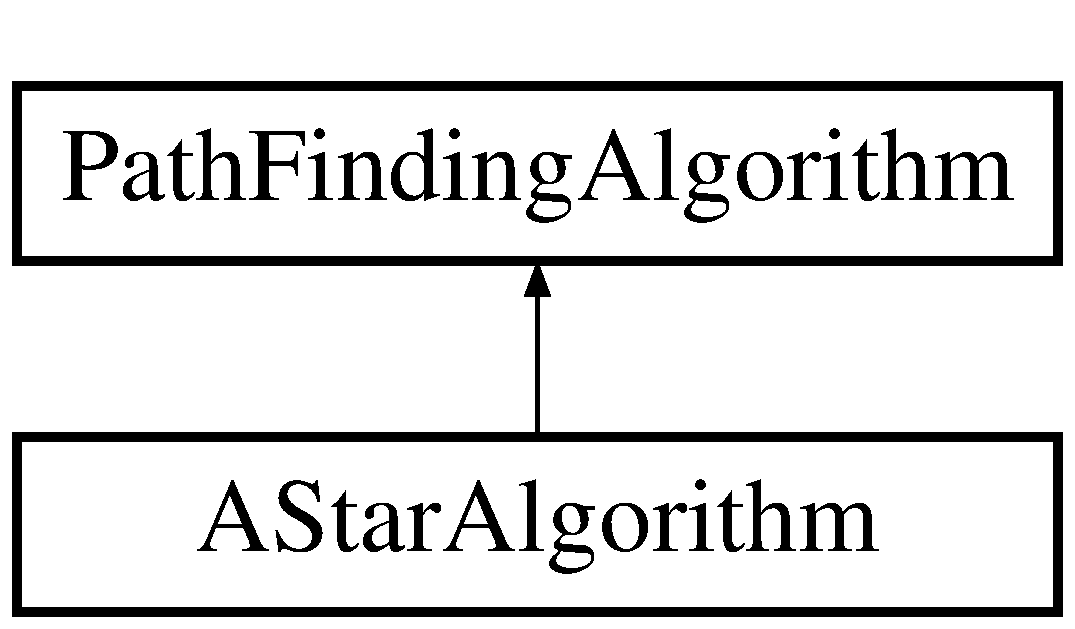
\includegraphics[height=2.000000cm]{d7/df1/classPathFindingAlgorithm}
\end{center}
\end{figure}
\subsection*{Public Member Functions}
\begin{DoxyCompactItemize}
\item 
\hyperlink{classPathFindingAlgorithm_ad9af1fa0b8bb6dc6660219c0b21a3749}{Path\-Finding\-Algorithm} ()
\begin{DoxyCompactList}\small\item\em Constructor of \hyperlink{classPathFindingAlgorithm}{Path\-Finding\-Algorithm} class. \end{DoxyCompactList}\item 
\hyperlink{classPathFindingAlgorithm_a68fdd88d9348febf0e1814af9add5ca3}{$\sim$\-Path\-Finding\-Algorithm} ()
\begin{DoxyCompactList}\small\item\em Deconstructor of \hyperlink{classPathFindingAlgorithm}{Path\-Finding\-Algorithm} class. \end{DoxyCompactList}\item 
void \hyperlink{classPathFindingAlgorithm_a31b4a12fa7164f0f71649f0505c8031e}{init} ()
\begin{DoxyCompactList}\small\item\em Initialize map and graph node, edges. \end{DoxyCompactList}\item 
void \hyperlink{classPathFindingAlgorithm_a71b876665f35f458137ff9f2347fcc54}{build\-Graph} ()
\begin{DoxyCompactList}\small\item\em Build graph by storing map info into nodes and edges for finding shortest path. \end{DoxyCompactList}\item 
void \hyperlink{classPathFindingAlgorithm_a334c5cfc5b40a1e8458eb960ff5f541c}{reconstruct\-Path} (\hyperlink{classNode}{Node} $\ast$)
\begin{DoxyCompactList}\small\item\em Reconstruct graph by traversing from goal to start via parent\-Index of nodes and store the path indices in member path which is a vector of integers. \end{DoxyCompactList}\item 
bool \hyperlink{classPathFindingAlgorithm_a2b48e12615aecc6fd952efcb5d920864}{set\-Param} (int, int)
\begin{DoxyCompactList}\small\item\em Set start and goal indices. \end{DoxyCompactList}\item 
void \hyperlink{classPathFindingAlgorithm_a98a59e7a6797895ac08be283850ab534}{output\-Path} (int)
\begin{DoxyCompactList}\small\item\em Output path in map. \end{DoxyCompactList}\item 
void \hyperlink{classPathFindingAlgorithm_a836f5c7fd0ea0e2201ed954f55ca523b}{output\-Map} ()
\begin{DoxyCompactList}\small\item\em Output map with indices on screen. \end{DoxyCompactList}\item 
virtual void \hyperlink{classPathFindingAlgorithm_adbd9dfe9d49577e9420669f59c290f55}{comput\-Path} ()
\begin{DoxyCompactList}\small\item\em Virtual function of finding shortest path. \end{DoxyCompactList}\item 
std\-::vector$<$ int $>$ \hyperlink{classPathFindingAlgorithm_a2c614eeead913e62288faa5499467529}{get\-Path} ()
\begin{DoxyCompactList}\small\item\em Get shotest path indices from start to goal. \end{DoxyCompactList}\item 
double \hyperlink{classPathFindingAlgorithm_a0c0eaaa84d7739a3c09ad012b37e8bd9}{get\-Total\-Cost} ()
\begin{DoxyCompactList}\small\item\em Get total cost of shortest path. \end{DoxyCompactList}\item 
int \hyperlink{classPathFindingAlgorithm_a6d2b42a027cd39039861f148cbf624f0}{get\-Steps} ()
\begin{DoxyCompactList}\small\item\em Get steps taken to find the shortest path. \end{DoxyCompactList}\end{DoxyCompactItemize}
\subsection*{Protected Attributes}
\begin{DoxyCompactItemize}
\item 
std\-::vector$<$ \hyperlink{classNode}{Node} $>$ \hyperlink{classPathFindingAlgorithm_a3405321350d5fb10ba367c47944a7b77}{nodes}
\begin{DoxyCompactList}\small\item\em vector of nodes \end{DoxyCompactList}\item 
std\-::vector$<$ \hyperlink{classEdge}{Edge} $>$ \hyperlink{classPathFindingAlgorithm_ae535e0897714e84f5ab40d5dc5d654ec}{edges}
\begin{DoxyCompactList}\small\item\em vector of edges \end{DoxyCompactList}\item 
int \hyperlink{classPathFindingAlgorithm_a1c31bd6b8c57459c32ada19cf9bf412a}{start}
\begin{DoxyCompactList}\small\item\em start index \end{DoxyCompactList}\item 
int \hyperlink{classPathFindingAlgorithm_ae8acf41f92ba72a969a44640c99fb8a4}{goal}
\begin{DoxyCompactList}\small\item\em goal index \end{DoxyCompactList}\item 
double \hyperlink{classPathFindingAlgorithm_ad6a91f82618d6a7a95900b5c63337837}{total\-Cost}
\begin{DoxyCompactList}\small\item\em cost of shortest path \end{DoxyCompactList}\item 
int \hyperlink{classPathFindingAlgorithm_aa4d442ba7d2499f61e81b8c0fabc55a5}{steps}
\begin{DoxyCompactList}\small\item\em steps to find shortest path \end{DoxyCompactList}\item 
std\-::vector$<$ int $>$ \hyperlink{classPathFindingAlgorithm_ab177b2276cdf28fb77361bff19745b17}{path}
\begin{DoxyCompactList}\small\item\em indices of shortest path \end{DoxyCompactList}\end{DoxyCompactItemize}


\subsection{Detailed Description}
Class that implements the basic functions reqiured for path finding algorithm. 

\subsection{Constructor \& Destructor Documentation}
\hypertarget{classPathFindingAlgorithm_ad9af1fa0b8bb6dc6660219c0b21a3749}{\index{Path\-Finding\-Algorithm@{Path\-Finding\-Algorithm}!Path\-Finding\-Algorithm@{Path\-Finding\-Algorithm}}
\index{Path\-Finding\-Algorithm@{Path\-Finding\-Algorithm}!PathFindingAlgorithm@{Path\-Finding\-Algorithm}}
\subsubsection[{Path\-Finding\-Algorithm}]{\setlength{\rightskip}{0pt plus 5cm}Path\-Finding\-Algorithm\-::\-Path\-Finding\-Algorithm (
\begin{DoxyParamCaption}
{}
\end{DoxyParamCaption}
)\hspace{0.3cm}{\ttfamily [inline]}}}\label{classPathFindingAlgorithm_ad9af1fa0b8bb6dc6660219c0b21a3749}


Constructor of \hyperlink{classPathFindingAlgorithm}{Path\-Finding\-Algorithm} class. 


\begin{DoxyParams}{Parameters}
{\em none} & \\
\hline
\end{DoxyParams}
\begin{DoxyReturn}{Returns}
none 
\end{DoxyReturn}

\begin{DoxyCode}
60 \{\}
\end{DoxyCode}
\hypertarget{classPathFindingAlgorithm_a68fdd88d9348febf0e1814af9add5ca3}{\index{Path\-Finding\-Algorithm@{Path\-Finding\-Algorithm}!$\sim$\-Path\-Finding\-Algorithm@{$\sim$\-Path\-Finding\-Algorithm}}
\index{$\sim$\-Path\-Finding\-Algorithm@{$\sim$\-Path\-Finding\-Algorithm}!PathFindingAlgorithm@{Path\-Finding\-Algorithm}}
\subsubsection[{$\sim$\-Path\-Finding\-Algorithm}]{\setlength{\rightskip}{0pt plus 5cm}Path\-Finding\-Algorithm\-::$\sim$\-Path\-Finding\-Algorithm (
\begin{DoxyParamCaption}
{}
\end{DoxyParamCaption}
)\hspace{0.3cm}{\ttfamily [inline]}}}\label{classPathFindingAlgorithm_a68fdd88d9348febf0e1814af9add5ca3}


Deconstructor of \hyperlink{classPathFindingAlgorithm}{Path\-Finding\-Algorithm} class. 


\begin{DoxyParams}{Parameters}
{\em none} & \\
\hline
\end{DoxyParams}
\begin{DoxyReturn}{Returns}
none 
\end{DoxyReturn}

\begin{DoxyCode}
69 \{\}
\end{DoxyCode}


\subsection{Member Function Documentation}
\hypertarget{classPathFindingAlgorithm_a71b876665f35f458137ff9f2347fcc54}{\index{Path\-Finding\-Algorithm@{Path\-Finding\-Algorithm}!build\-Graph@{build\-Graph}}
\index{build\-Graph@{build\-Graph}!PathFindingAlgorithm@{Path\-Finding\-Algorithm}}
\subsubsection[{build\-Graph}]{\setlength{\rightskip}{0pt plus 5cm}void Path\-Finding\-Algorithm\-::build\-Graph (
\begin{DoxyParamCaption}
\item[{void}]{}
\end{DoxyParamCaption}
)}}\label{classPathFindingAlgorithm_a71b876665f35f458137ff9f2347fcc54}


Build graph by storing map info into nodes and edges for finding shortest path. 


\begin{DoxyParams}{Parameters}
{\em none} & \\
\hline
\end{DoxyParams}
\begin{DoxyReturn}{Returns}
none 
\end{DoxyReturn}

\begin{DoxyCode}
64                                           \{
65 
66     vector<int>* mapArray = \textcolor{keyword}{nullptr};
67 
68     \textcolor{keywordtype}{int}* dir = \textcolor{keyword}{nullptr};
69     \textcolor{keywordtype}{int} i = 0;
70     \textcolor{keywordtype}{int} j = 0;
71     \textcolor{keywordtype}{int} k = 0;
72     \textcolor{keywordtype}{int} index = 1;
73     
74     \textcolor{comment}{// cout << endl << "PathFindingAlgorithm::BuildGraph" << endl;}
75     
76     mapArray = map.\hyperlink{classMap_ad5c4312f11909eafc091715686b6ceda}{getMap}();
77     \textcolor{keywordflow}{if} (mapArray == \textcolor{keyword}{nullptr})
78         \textcolor{keywordflow}{return};
79 
80     dir = map.\hyperlink{classMap_a4f9142718a50c64152465aacc1033f26}{getMoveDir}();
81     \textcolor{keywordflow}{if} (dir == \textcolor{keyword}{nullptr})
82         \textcolor{keywordflow}{return};
83 
84     \textcolor{comment}{// cout << "Generating nodes" << endl;}
85 
86 
87     \textcolor{keywordtype}{int} n = map.\hyperlink{classMap_a80e0ea134ccb9a22092ce4c520063cd2}{getRow}();
88     \textcolor{keywordtype}{int} m = map.\hyperlink{classMap_a88d24c08a4669040d7de6bd5f6272862}{getCol}();
89 
90 
91     \textcolor{comment}{// cout << "map row " << n << endl;}
92     \textcolor{comment}{// cout << "map column " << m << endl;}
93 
94     \textcolor{comment}{// generate nodes}
95     \textcolor{keywordflow}{for} (i = 0, index = 1; i < n; ++i) \{ \textcolor{comment}{// row, y}
96         \textcolor{keywordflow}{for} (j = 0; j < m; ++j) \{ \textcolor{comment}{// column, x}
97             \textcolor{comment}{// create a node and add to node vector}
98 
99             \textcolor{comment}{// cout << index << " (" << i << ", " << j << ")" << endl;}
100         
101             \hyperlink{classPathFindingAlgorithm_a3405321350d5fb10ba367c47944a7b77}{nodes}.emplace\_back(index, i, j);
102             ++index;
103         \}
104     \}
105 
106     \textcolor{comment}{// cout << endl << "Generating edges" << endl;}
107 
108     \textcolor{comment}{// generate edges}
109     \textcolor{keywordflow}{for} (i = 0; i < n; ++i) \{ \textcolor{comment}{// row, y}
110         \textcolor{keywordflow}{for} (j = 0; j < m; ++j) \{ \textcolor{comment}{// column, x}
111 
112             \textcolor{keywordtype}{int} numDir = map.\hyperlink{classMap_a04501949c81ac8dd6a7aeaca908fe969}{getNumDir}();
113             \textcolor{keywordtype}{int} neighborX = 0;
114             \textcolor{keywordtype}{int} neighborY = 0;
115             \textcolor{keywordtype}{int} startIdx = 0;
116             \textcolor{keywordtype}{int} endIdx = 0;
117             \textcolor{keywordtype}{double} cost = 0;
118             \textcolor{keywordtype}{double} diagCost = 0;
119     
120             \textcolor{keywordflow}{for} (k = 0; k < numDir; ++k) \{
121                 neighborX = j + *(dir+k*2);
122                 neighborY = i + *(dir+k*2+1);
123 
124                 \textcolor{comment}{// cout << "(" << i << "," << j << ") (" << neighborX}
125                 \textcolor{comment}{// << "," << neighborY << ")" << endl;}
126 
127                 \textcolor{keywordflow}{if} ((neighborX >= 0) && (neighborY >= 0) &&
128                       (neighborX < m) && (neighborY < n)) \{
129                     \textcolor{comment}{// add node to edge list}
130                     startIdx = i * m + j + 1;
131                     endIdx = neighborY * m + neighborX + 1;
132 
133                     \textcolor{comment}{// set cost for moving between nodes}
134                     cost = (*mapArray)[endIdx-1];
135 
136                     \textcolor{comment}{// setting cost to 1.5x for diagonal movement}
137                     \textcolor{keywordflow}{if} ((k==0) || (k==2) || (k==5) || (k==7))
138                        diagCost = 1.5;
139                     \textcolor{keywordflow}{else}
140                        diagCost = 1.0;
141 
142                     \textcolor{keywordflow}{if} (cost < std::numeric\_limits<int>::max())
143                         cost = cost * diagCost;
144 
145                     \textcolor{comment}{// cout << k << " (" << startIdx << "," << endIdx << ") " << cost << endl;}
146 
147                     \hyperlink{classPathFindingAlgorithm_ae535e0897714e84f5ab40d5dc5d654ec}{edges}.emplace\_back(startIdx, endIdx, cost);
148                 \}
149             \}
150         \}
151     \}
152 
153     \textcolor{keywordflow}{return};
154 \}
\end{DoxyCode}
\hypertarget{classPathFindingAlgorithm_adbd9dfe9d49577e9420669f59c290f55}{\index{Path\-Finding\-Algorithm@{Path\-Finding\-Algorithm}!comput\-Path@{comput\-Path}}
\index{comput\-Path@{comput\-Path}!PathFindingAlgorithm@{Path\-Finding\-Algorithm}}
\subsubsection[{comput\-Path}]{\setlength{\rightskip}{0pt plus 5cm}virtual void Path\-Finding\-Algorithm\-::comput\-Path (
\begin{DoxyParamCaption}
{}
\end{DoxyParamCaption}
)\hspace{0.3cm}{\ttfamily [inline]}, {\ttfamily [virtual]}}}\label{classPathFindingAlgorithm_adbd9dfe9d49577e9420669f59c290f55}


Virtual function of finding shortest path. 


\begin{DoxyParams}{Parameters}
{\em none} & \\
\hline
\end{DoxyParams}
\begin{DoxyReturn}{Returns}
none 
\end{DoxyReturn}

\begin{DoxyCode}
139 \{\}
\end{DoxyCode}
\hypertarget{classPathFindingAlgorithm_a2c614eeead913e62288faa5499467529}{\index{Path\-Finding\-Algorithm@{Path\-Finding\-Algorithm}!get\-Path@{get\-Path}}
\index{get\-Path@{get\-Path}!PathFindingAlgorithm@{Path\-Finding\-Algorithm}}
\subsubsection[{get\-Path}]{\setlength{\rightskip}{0pt plus 5cm}std\-::vector$<$int$>$ Path\-Finding\-Algorithm\-::get\-Path (
\begin{DoxyParamCaption}
{}
\end{DoxyParamCaption}
)\hspace{0.3cm}{\ttfamily [inline]}}}\label{classPathFindingAlgorithm_a2c614eeead913e62288faa5499467529}


Get shotest path indices from start to goal. 


\begin{DoxyParams}{Parameters}
{\em none} & \\
\hline
\end{DoxyParams}
\begin{DoxyReturn}{Returns}
shortest path indices from start to goal in vector int 
\end{DoxyReturn}

\begin{DoxyCode}
149                            \{ \textcolor{keywordflow}{return} \hyperlink{classPathFindingAlgorithm_ab177b2276cdf28fb77361bff19745b17}{path}; \}
\end{DoxyCode}
\hypertarget{classPathFindingAlgorithm_a6d2b42a027cd39039861f148cbf624f0}{\index{Path\-Finding\-Algorithm@{Path\-Finding\-Algorithm}!get\-Steps@{get\-Steps}}
\index{get\-Steps@{get\-Steps}!PathFindingAlgorithm@{Path\-Finding\-Algorithm}}
\subsubsection[{get\-Steps}]{\setlength{\rightskip}{0pt plus 5cm}int Path\-Finding\-Algorithm\-::get\-Steps (
\begin{DoxyParamCaption}
{}
\end{DoxyParamCaption}
)\hspace{0.3cm}{\ttfamily [inline]}}}\label{classPathFindingAlgorithm_a6d2b42a027cd39039861f148cbf624f0}


Get steps taken to find the shortest path. 


\begin{DoxyParams}{Parameters}
{\em none} & \\
\hline
\end{DoxyParams}
\begin{DoxyReturn}{Returns}
steps taken to find shortest path in int 
\end{DoxyReturn}

\begin{DoxyCode}
167 \{ \textcolor{keywordflow}{return} \hyperlink{classPathFindingAlgorithm_aa4d442ba7d2499f61e81b8c0fabc55a5}{steps}; \}
\end{DoxyCode}
\hypertarget{classPathFindingAlgorithm_a0c0eaaa84d7739a3c09ad012b37e8bd9}{\index{Path\-Finding\-Algorithm@{Path\-Finding\-Algorithm}!get\-Total\-Cost@{get\-Total\-Cost}}
\index{get\-Total\-Cost@{get\-Total\-Cost}!PathFindingAlgorithm@{Path\-Finding\-Algorithm}}
\subsubsection[{get\-Total\-Cost}]{\setlength{\rightskip}{0pt plus 5cm}double Path\-Finding\-Algorithm\-::get\-Total\-Cost (
\begin{DoxyParamCaption}
{}
\end{DoxyParamCaption}
)\hspace{0.3cm}{\ttfamily [inline]}}}\label{classPathFindingAlgorithm_a0c0eaaa84d7739a3c09ad012b37e8bd9}


Get total cost of shortest path. 


\begin{DoxyParams}{Parameters}
{\em none} & \\
\hline
\end{DoxyParams}
\begin{DoxyReturn}{Returns}
total cost from start to goal in double 
\end{DoxyReturn}

\begin{DoxyCode}
159                 \{ \textcolor{keywordflow}{return} \hyperlink{classPathFindingAlgorithm_ad6a91f82618d6a7a95900b5c63337837}{totalCost}; \}
\end{DoxyCode}
\hypertarget{classPathFindingAlgorithm_a31b4a12fa7164f0f71649f0505c8031e}{\index{Path\-Finding\-Algorithm@{Path\-Finding\-Algorithm}!init@{init}}
\index{init@{init}!PathFindingAlgorithm@{Path\-Finding\-Algorithm}}
\subsubsection[{init}]{\setlength{\rightskip}{0pt plus 5cm}void Path\-Finding\-Algorithm\-::init (
\begin{DoxyParamCaption}
\item[{void}]{}
\end{DoxyParamCaption}
)}}\label{classPathFindingAlgorithm_a31b4a12fa7164f0f71649f0505c8031e}


Initialize map and graph node, edges. 


\begin{DoxyParams}{Parameters}
{\em none} & \\
\hline
\end{DoxyParams}
\begin{DoxyReturn}{Returns}
none 
\end{DoxyReturn}

\begin{DoxyCode}
54                                     \{
55     \hyperlink{classPathFindingAlgorithm_a3405321350d5fb10ba367c47944a7b77}{nodes}.clear();
56     \hyperlink{classPathFindingAlgorithm_ae535e0897714e84f5ab40d5dc5d654ec}{edges}.clear();
57     \hyperlink{classPathFindingAlgorithm_ab177b2276cdf28fb77361bff19745b17}{path}.clear();
58 
59     map.\hyperlink{classMap_a389e4f5c49c1a33e9c0e6c4b2f0605ed}{createMap}(\hyperlink{PathFindAlgorithm_8hpp_a766bf3e65d7bed0d203a77d49e17d66b}{DEFAUTL\_INPUT\_MAP});
60     \hyperlink{classPathFindingAlgorithm_a71b876665f35f458137ff9f2347fcc54}{buildGraph}();
61 \}
\end{DoxyCode}
\hypertarget{classPathFindingAlgorithm_a836f5c7fd0ea0e2201ed954f55ca523b}{\index{Path\-Finding\-Algorithm@{Path\-Finding\-Algorithm}!output\-Map@{output\-Map}}
\index{output\-Map@{output\-Map}!PathFindingAlgorithm@{Path\-Finding\-Algorithm}}
\subsubsection[{output\-Map}]{\setlength{\rightskip}{0pt plus 5cm}void Path\-Finding\-Algorithm\-::output\-Map (
\begin{DoxyParamCaption}
{}
\end{DoxyParamCaption}
)}}\label{classPathFindingAlgorithm_a836f5c7fd0ea0e2201ed954f55ca523b}


Output map with indices on screen. 


\begin{DoxyParams}{Parameters}
{\em none} & \\
\hline
\end{DoxyParams}
\begin{DoxyReturn}{Returns}
none 
\end{DoxyReturn}

\begin{DoxyCode}
226                                      \{
227 
228     map.\hyperlink{classMap_ac5af28a5fed55d9ca5d1dab5cb9f3f9c}{displayMap}();
229     \textcolor{keywordflow}{return};
230 \}
\end{DoxyCode}
\hypertarget{classPathFindingAlgorithm_a98a59e7a6797895ac08be283850ab534}{\index{Path\-Finding\-Algorithm@{Path\-Finding\-Algorithm}!output\-Path@{output\-Path}}
\index{output\-Path@{output\-Path}!PathFindingAlgorithm@{Path\-Finding\-Algorithm}}
\subsubsection[{output\-Path}]{\setlength{\rightskip}{0pt plus 5cm}void Path\-Finding\-Algorithm\-::output\-Path (
\begin{DoxyParamCaption}
\item[{int}]{option}
\end{DoxyParamCaption}
)}}\label{classPathFindingAlgorithm_a98a59e7a6797895ac08be283850ab534}


Output path in map. 


\begin{DoxyParams}{Parameters}
{\em option} & to output path in int \par
 0\-: display path in map on screen \par
 1\-: output path in map to file \par
 2\-: both display path in map on screen and save to file \\
\hline
\end{DoxyParams}
\begin{DoxyReturn}{Returns}
none 
\end{DoxyReturn}

\begin{DoxyCode}
204                                                 \{
205 
206     \textcolor{keywordflow}{switch}(option) \{
207          \textcolor{comment}{// display map on screen}
208         \textcolor{keywordflow}{case} 0:
209             map.\hyperlink{classMap_a4358aea9eb9f207aae23fc8d9a40b97a}{displayPath}(\hyperlink{classPathFindingAlgorithm_ab177b2276cdf28fb77361bff19745b17}{path});
210             \textcolor{keywordflow}{break};
211 
212         \textcolor{comment}{// output to file}
213         \textcolor{keywordflow}{case} 1:
214             map.\hyperlink{classMap_a43ce2c046c7908d95e06bd29182ac6bf}{saveMap}(\hyperlink{PathFindAlgorithm_8hpp_aaac5b5627661fef63e64ce61808f30f8}{DEFAUTL\_OUTPUT\_MAP}, \hyperlink{classPathFindingAlgorithm_ab177b2276cdf28fb77361bff19745b17}{path});
215             \textcolor{keywordflow}{break};
216 
217         \textcolor{keywordflow}{case} 2:
218         \textcolor{keywordflow}{default}:
219             map.\hyperlink{classMap_a4358aea9eb9f207aae23fc8d9a40b97a}{displayPath}(\hyperlink{classPathFindingAlgorithm_ab177b2276cdf28fb77361bff19745b17}{path});
220             map.\hyperlink{classMap_a43ce2c046c7908d95e06bd29182ac6bf}{saveMap}(\hyperlink{PathFindAlgorithm_8hpp_aaac5b5627661fef63e64ce61808f30f8}{DEFAUTL\_OUTPUT\_MAP}, \hyperlink{classPathFindingAlgorithm_ab177b2276cdf28fb77361bff19745b17}{path});
221             \textcolor{keywordflow}{break};
222     \}
223 \}
\end{DoxyCode}
\hypertarget{classPathFindingAlgorithm_a334c5cfc5b40a1e8458eb960ff5f541c}{\index{Path\-Finding\-Algorithm@{Path\-Finding\-Algorithm}!reconstruct\-Path@{reconstruct\-Path}}
\index{reconstruct\-Path@{reconstruct\-Path}!PathFindingAlgorithm@{Path\-Finding\-Algorithm}}
\subsubsection[{reconstruct\-Path}]{\setlength{\rightskip}{0pt plus 5cm}void Path\-Finding\-Algorithm\-::reconstruct\-Path (
\begin{DoxyParamCaption}
\item[{{\bf Node} $\ast$}]{node}
\end{DoxyParamCaption}
)}}\label{classPathFindingAlgorithm_a334c5cfc5b40a1e8458eb960ff5f541c}


Reconstruct graph by traversing from goal to start via parent\-Index of nodes and store the path indices in member path which is a vector of integers. 


\begin{DoxyParams}{Parameters}
{\em \hyperlink{classNode}{Node}} & pointer of goal \\
\hline
\end{DoxyParams}
\begin{DoxyReturn}{Returns}
none 
\end{DoxyReturn}

\begin{DoxyCode}
157                                                      \{
158     list<Node*> tempPath;
159     \hyperlink{classNode}{Node} *temp = node;
160 
161     \textcolor{keywordflow}{if} (temp == \textcolor{keyword}{nullptr})
162         \textcolor{keywordflow}{return};
163 
164     \textcolor{comment}{// reconstruct path using node's parent pointer}
165     \textcolor{keywordflow}{while} (temp != \textcolor{keyword}{nullptr}) \{
166         \textcolor{comment}{// add the start node and break}
167         \textcolor{keywordflow}{if} (temp->\hyperlink{classNode_a38525d55d0f15d4b6be0b3b8ed150441}{getParentIndex}() == 0) \{
168             tempPath.emplace\_front(temp);
169             \textcolor{keywordflow}{break};
170         \}
171 
172         tempPath.emplace\_front(temp);
173         temp = &\hyperlink{classPathFindingAlgorithm_a3405321350d5fb10ba367c47944a7b77}{nodes}[temp->\hyperlink{classNode_a38525d55d0f15d4b6be0b3b8ed150441}{getParentIndex}()-1];
174     \}
175 
176 
177     \textcolor{comment}{// cout << "Shortest Path: ";}
178 
179     \textcolor{comment}{// save into vector from start to goal}
180     \textcolor{keywordflow}{for} (\textcolor{keyword}{auto}& n : tempPath) \{
181         \textcolor{comment}{// cout << n->getIndex() << " ";}
182         \hyperlink{classPathFindingAlgorithm_ab177b2276cdf28fb77361bff19745b17}{path}.emplace\_back(n->getIndex());
183     \}
184 
185     \textcolor{comment}{// cout << endl;}
186 
187 
188     \textcolor{keywordflow}{return};
189 \}
\end{DoxyCode}
\hypertarget{classPathFindingAlgorithm_a2b48e12615aecc6fd952efcb5d920864}{\index{Path\-Finding\-Algorithm@{Path\-Finding\-Algorithm}!set\-Param@{set\-Param}}
\index{set\-Param@{set\-Param}!PathFindingAlgorithm@{Path\-Finding\-Algorithm}}
\subsubsection[{set\-Param}]{\setlength{\rightskip}{0pt plus 5cm}bool Path\-Finding\-Algorithm\-::set\-Param (
\begin{DoxyParamCaption}
\item[{int}]{s, }
\item[{int}]{g}
\end{DoxyParamCaption}
)}}\label{classPathFindingAlgorithm_a2b48e12615aecc6fd952efcb5d920864}


Set start and goal indices. 


\begin{DoxyParams}{Parameters}
{\em start} & node index in int \\
\hline
{\em goal} & node index in int \\
\hline
\end{DoxyParams}
\begin{DoxyReturn}{Returns}
true if start, goal are within map range and are not obstacle nodes, false otherwise 
\end{DoxyReturn}

\begin{DoxyCode}
192                                                 \{
193     \textcolor{comment}{// set start and goal indices}
194     \textcolor{keywordflow}{if} (map.\hyperlink{classMap_aa64162f950a1936e1eaf42609e091524}{setStartGoal}(s, g)) \{
195         \hyperlink{classPathFindingAlgorithm_a1c31bd6b8c57459c32ada19cf9bf412a}{start} = s;
196         \hyperlink{classPathFindingAlgorithm_ae8acf41f92ba72a969a44640c99fb8a4}{goal} = g;
197         \textcolor{keywordflow}{return} \textcolor{keyword}{true};
198     \} \textcolor{keywordflow}{else} \{
199         \textcolor{keywordflow}{return} \textcolor{keyword}{false};
200     \}
201 \}
\end{DoxyCode}


\subsection{Member Data Documentation}
\hypertarget{classPathFindingAlgorithm_ae535e0897714e84f5ab40d5dc5d654ec}{\index{Path\-Finding\-Algorithm@{Path\-Finding\-Algorithm}!edges@{edges}}
\index{edges@{edges}!PathFindingAlgorithm@{Path\-Finding\-Algorithm}}
\subsubsection[{edges}]{\setlength{\rightskip}{0pt plus 5cm}std\-::vector$<${\bf Edge}$>$ Path\-Finding\-Algorithm\-::edges\hspace{0.3cm}{\ttfamily [protected]}}}\label{classPathFindingAlgorithm_ae535e0897714e84f5ab40d5dc5d654ec}


vector of edges 

\hypertarget{classPathFindingAlgorithm_ae8acf41f92ba72a969a44640c99fb8a4}{\index{Path\-Finding\-Algorithm@{Path\-Finding\-Algorithm}!goal@{goal}}
\index{goal@{goal}!PathFindingAlgorithm@{Path\-Finding\-Algorithm}}
\subsubsection[{goal}]{\setlength{\rightskip}{0pt plus 5cm}int Path\-Finding\-Algorithm\-::goal\hspace{0.3cm}{\ttfamily [protected]}}}\label{classPathFindingAlgorithm_ae8acf41f92ba72a969a44640c99fb8a4}


goal index 

\hypertarget{classPathFindingAlgorithm_a3405321350d5fb10ba367c47944a7b77}{\index{Path\-Finding\-Algorithm@{Path\-Finding\-Algorithm}!nodes@{nodes}}
\index{nodes@{nodes}!PathFindingAlgorithm@{Path\-Finding\-Algorithm}}
\subsubsection[{nodes}]{\setlength{\rightskip}{0pt plus 5cm}std\-::vector$<${\bf Node}$>$ Path\-Finding\-Algorithm\-::nodes\hspace{0.3cm}{\ttfamily [protected]}}}\label{classPathFindingAlgorithm_a3405321350d5fb10ba367c47944a7b77}


vector of nodes 

\hypertarget{classPathFindingAlgorithm_ab177b2276cdf28fb77361bff19745b17}{\index{Path\-Finding\-Algorithm@{Path\-Finding\-Algorithm}!path@{path}}
\index{path@{path}!PathFindingAlgorithm@{Path\-Finding\-Algorithm}}
\subsubsection[{path}]{\setlength{\rightskip}{0pt plus 5cm}std\-::vector$<$int$>$ Path\-Finding\-Algorithm\-::path\hspace{0.3cm}{\ttfamily [protected]}}}\label{classPathFindingAlgorithm_ab177b2276cdf28fb77361bff19745b17}


indices of shortest path 

\hypertarget{classPathFindingAlgorithm_a1c31bd6b8c57459c32ada19cf9bf412a}{\index{Path\-Finding\-Algorithm@{Path\-Finding\-Algorithm}!start@{start}}
\index{start@{start}!PathFindingAlgorithm@{Path\-Finding\-Algorithm}}
\subsubsection[{start}]{\setlength{\rightskip}{0pt plus 5cm}int Path\-Finding\-Algorithm\-::start\hspace{0.3cm}{\ttfamily [protected]}}}\label{classPathFindingAlgorithm_a1c31bd6b8c57459c32ada19cf9bf412a}


start index 

\hypertarget{classPathFindingAlgorithm_aa4d442ba7d2499f61e81b8c0fabc55a5}{\index{Path\-Finding\-Algorithm@{Path\-Finding\-Algorithm}!steps@{steps}}
\index{steps@{steps}!PathFindingAlgorithm@{Path\-Finding\-Algorithm}}
\subsubsection[{steps}]{\setlength{\rightskip}{0pt plus 5cm}int Path\-Finding\-Algorithm\-::steps\hspace{0.3cm}{\ttfamily [protected]}}}\label{classPathFindingAlgorithm_aa4d442ba7d2499f61e81b8c0fabc55a5}


steps to find shortest path 

\hypertarget{classPathFindingAlgorithm_ad6a91f82618d6a7a95900b5c63337837}{\index{Path\-Finding\-Algorithm@{Path\-Finding\-Algorithm}!total\-Cost@{total\-Cost}}
\index{total\-Cost@{total\-Cost}!PathFindingAlgorithm@{Path\-Finding\-Algorithm}}
\subsubsection[{total\-Cost}]{\setlength{\rightskip}{0pt plus 5cm}double Path\-Finding\-Algorithm\-::total\-Cost\hspace{0.3cm}{\ttfamily [protected]}}}\label{classPathFindingAlgorithm_ad6a91f82618d6a7a95900b5c63337837}


cost of shortest path 



The documentation for this class was generated from the following files\-:\begin{DoxyCompactItemize}
\item 
include/\hyperlink{PathFindAlgorithm_8hpp}{Path\-Find\-Algorithm.\-hpp}\item 
app/\hyperlink{PathFindAlgorithm_8cpp}{Path\-Find\-Algorithm.\-cpp}\end{DoxyCompactItemize}

\chapter{File Documentation}
\hypertarget{AStarAlgorithm_8cpp}{\section{app/\-A\-Star\-Algorithm.cpp File Reference}
\label{AStarAlgorithm_8cpp}\index{app/\-A\-Star\-Algorithm.\-cpp@{app/\-A\-Star\-Algorithm.\-cpp}}
}


Implementation of class \hyperlink{classAStarAlgorithm}{A\-Star\-Algorithm} methods.  


{\ttfamily \#include \char`\"{}A\-Star\-Algorithm.\-hpp\char`\"{}}\\*
{\ttfamily \#include $<$math.\-h$>$}\\*
{\ttfamily \#include $<$iostream$>$}\\*
{\ttfamily \#include $<$limits$>$}\\*
\subsection*{Functions}
\begin{DoxyCompactItemize}
\item 
bool \hyperlink{AStarAlgorithm_8cpp_a79d7a8f837b09f62b8595c351f24f367}{check\-List} (int index, list$<$ \hyperlink{classNode}{Node} $\ast$ $>$ const \&nodes)
\item 
bool \hyperlink{AStarAlgorithm_8cpp_a9941f2d9671bce063d16ba2ecd046d6a}{compare\-Cost} (\hyperlink{classNode}{Node} $\ast$first, \hyperlink{classNode}{Node} $\ast$second)
\end{DoxyCompactItemize}


\subsection{Detailed Description}
Implementation of class \hyperlink{classAStarAlgorithm}{A\-Star\-Algorithm} methods. This file implements class \hyperlink{classAStarAlgorithm}{A\-Star\-Algorithm} methods and its helper functions.

\hyperlink{classAStarAlgorithm}{A\-Star\-Algorithm} derives from Path\-Find\-Algorithm class and implements virtual function Comput\-Path to compute shortest path using A star algorithm. The heuristic estimation used in A star algorithm here is implemented using Euclidean distance.

\begin{DoxyAuthor}{Author}
Huei Tzu Tsai 
\end{DoxyAuthor}
\begin{DoxyDate}{Date}
03/07/2017 
\end{DoxyDate}


\subsection{Function Documentation}
\hypertarget{AStarAlgorithm_8cpp_a79d7a8f837b09f62b8595c351f24f367}{\index{A\-Star\-Algorithm.\-cpp@{A\-Star\-Algorithm.\-cpp}!check\-List@{check\-List}}
\index{check\-List@{check\-List}!AStarAlgorithm.cpp@{A\-Star\-Algorithm.\-cpp}}
\subsubsection[{check\-List}]{\setlength{\rightskip}{0pt plus 5cm}bool check\-List (
\begin{DoxyParamCaption}
\item[{int}]{index, }
\item[{list$<$ {\bf Node} $\ast$ $>$ const \&}]{nodes}
\end{DoxyParamCaption}
)}}\label{AStarAlgorithm_8cpp_a79d7a8f837b09f62b8595c351f24f367}

\begin{DoxyCode}
229                                                     \{
230     \textcolor{keywordtype}{bool} found = \textcolor{keyword}{false};
231 
232     \textcolor{keywordflow}{for} (\textcolor{keyword}{auto}& n : nodes) \{
233         \textcolor{keywordflow}{if} (n->getIndex() == index) \{
234             found = \textcolor{keyword}{true};
235             \textcolor{keywordflow}{break};
236         \}
237     \}
238 
239     \textcolor{keywordflow}{return} found;
240 \}
\end{DoxyCode}
\hypertarget{AStarAlgorithm_8cpp_a9941f2d9671bce063d16ba2ecd046d6a}{\index{A\-Star\-Algorithm.\-cpp@{A\-Star\-Algorithm.\-cpp}!compare\-Cost@{compare\-Cost}}
\index{compare\-Cost@{compare\-Cost}!AStarAlgorithm.cpp@{A\-Star\-Algorithm.\-cpp}}
\subsubsection[{compare\-Cost}]{\setlength{\rightskip}{0pt plus 5cm}bool compare\-Cost (
\begin{DoxyParamCaption}
\item[{{\bf Node} $\ast$}]{first, }
\item[{{\bf Node} $\ast$}]{second}
\end{DoxyParamCaption}
)}}\label{AStarAlgorithm_8cpp_a9941f2d9671bce063d16ba2ecd046d6a}

\begin{DoxyCode}
243                                             \{
244     \textcolor{keywordflow}{if} (first->\hyperlink{classNode_a9c7e1456a27ec44e98d75ca1d2db21f1}{getEstimateCost}() < second->\hyperlink{classNode_a9c7e1456a27ec44e98d75ca1d2db21f1}{getEstimateCost}())
245         \textcolor{keywordflow}{return} \textcolor{keyword}{true};
246     \textcolor{keywordflow}{else}
247         \textcolor{keywordflow}{return} \textcolor{keyword}{false};
248 \}
\end{DoxyCode}

\hypertarget{app_2main_8cpp}{\section{app/main.cpp File Reference}
\label{app_2main_8cpp}\index{app/main.\-cpp@{app/main.\-cpp}}
}
{\ttfamily \#include $<$iostream$>$}\\*
{\ttfamily \#include $<$string$>$}\\*
{\ttfamily \#include $<$vector$>$}\\*
{\ttfamily \#include \char`\"{}A\-Star\-Algorithm.\-hpp\char`\"{}}\\*
\subsection*{Functions}
\begin{DoxyCompactItemize}
\item 
int \hyperlink{app_2main_8cpp_a840291bc02cba5474a4cb46a9b9566fe}{main} (void)
\end{DoxyCompactItemize}


\subsection{Function Documentation}
\hypertarget{app_2main_8cpp_a840291bc02cba5474a4cb46a9b9566fe}{\index{app/main.\-cpp@{app/main.\-cpp}!main@{main}}
\index{main@{main}!app/main.cpp@{app/main.\-cpp}}
\subsubsection[{main}]{\setlength{\rightskip}{0pt plus 5cm}int main (
\begin{DoxyParamCaption}
\item[{void}]{}
\end{DoxyParamCaption}
)}}\label{app_2main_8cpp_a840291bc02cba5474a4cb46a9b9566fe}

\begin{DoxyCode}
59                \{
60     \textcolor{keywordtype}{string} mapFile;
61     \textcolor{keywordtype}{int} start = 1;
62     \textcolor{keywordtype}{int} goal = 2;
63     \textcolor{keywordtype}{int} option = 0;
64     \textcolor{keywordtype}{double} weight = 0.0;
65     vector<int> path;
66     \hyperlink{classAStarAlgorithm}{AStarAlgorithm} aStar;
67 
68     cout << \textcolor{stringliteral}{"Please enter map path (or ctl+d to use default):"} << endl;
69 
70     cin >> mapFile;
71     cin.clear();
72 
73     \textcolor{keywordflow}{if} (mapFile.empty())
74         mapFile = \hyperlink{PathFindAlgorithm_8hpp_a3fc18846efd2be281ed37ed05956a6de}{DEFAUTL\_DEFAULT\_MAP};
75 
76     \textcolor{keywordflow}{if} (!aStar.PathFindingAlgorithm::init(mapFile)) \{
77         cout << \textcolor{stringliteral}{"Fail to read map.  Please try again or use default map."}
78              << endl;
79         \textcolor{keywordflow}{return} -1;
80     \}
81 
82     aStar.PathFindingAlgorithm::outputMap();
83 
84     cout << \textcolor{stringliteral}{"Please enter start, goal indices"} << endl;
85 
86     cin >> start >> goal;
87     cin.clear();
88 
89     cout << \textcolor{stringliteral}{"start is "} << start << endl;
90     cout << \textcolor{stringliteral}{"goal is "} << goal << endl;
91 
92     \textcolor{keywordflow}{if} (aStar.PathFindingAlgorithm::setParam(start, goal) == \textcolor{keyword}{false}) \{
93         cout << \textcolor{stringliteral}{"Start or goal is out of map or obstacle, please try again."}
94              << endl;
95         \textcolor{keywordflow}{return} -1;
96     \}
97 
98     weight = 0.0;
99 
100     \textcolor{keywordflow}{if} (!aStar.\hyperlink{classAStarAlgorithm_af3adf65228c56523489d3bd4e278e66f}{computPath}(weight)) \{
101         cout << \textcolor{stringliteral}{"Fail to find path"} << endl;
102         \textcolor{keywordflow}{return} -1;
103     \}
104 
105     path = aStar.PathFindingAlgorithm::getPath();
106     cout << \textcolor{stringliteral}{"Dijkstra's Shortest Path:"};
107 
108     \textcolor{comment}{// save into vector from start to goal}
109     \textcolor{keywordflow}{for} (\textcolor{keyword}{auto}& n : path) \{
110         cout <<  \textcolor{stringliteral}{" "} << n;
111     \}
112     cout << endl;
113 
114     cout << \textcolor{stringliteral}{"Dijkstra's total cost is "}
115          << aStar.PathFindingAlgorithm::getTotalCost() << endl;
116 
117     cout << \textcolor{stringliteral}{"Dijkstra's total step is "}
118          << aStar.PathFindingAlgorithm::getSteps() << endl;
119 
120     \textcolor{comment}{// Init again to clear variables}
121     aStar.PathFindingAlgorithm::init(mapFile);
122     path.clear();
123 
124     \textcolor{comment}{// Compute using A star}
125     weight = 1.0;
126     \textcolor{keywordflow}{if} (!aStar.\hyperlink{classAStarAlgorithm_af3adf65228c56523489d3bd4e278e66f}{computPath}(weight)) \{
127         cout << \textcolor{stringliteral}{"Fail to find path"} << endl;
128         \textcolor{keywordflow}{return} -1;
129     \}
130 
131     path = aStar.PathFindingAlgorithm::getPath();
132     cout << \textcolor{stringliteral}{"A Star Shortest Path:"};
133 
134     \textcolor{comment}{// save into vector from start to goal}
135     \textcolor{keywordflow}{for} (\textcolor{keyword}{auto}& n : path) \{
136         cout <<  \textcolor{stringliteral}{" "} << n;
137     \}
138     cout << endl;
139 
140     cout << \textcolor{stringliteral}{"A Star total cost is "}
141          << aStar.PathFindingAlgorithm::getTotalCost() << endl;
142 
143     cout << \textcolor{stringliteral}{"A Star total step is "} << aStar.PathFindingAlgorithm::getSteps()
144          << endl;
145 
146     cout << \textcolor{stringliteral}{"Output A Star Path Option:"} << endl;
147     cout << \textcolor{stringliteral}{"0: path in map on screen"} << endl;
148     cout << \textcolor{stringliteral}{"1: path output to "} << \hyperlink{PathFindAlgorithm_8hpp_a2fa4f0a512b2d876f34e9aec1765d791}{DEFAUTL\_OUTPUT\_PATH} << endl;
149     cout << \textcolor{stringliteral}{"   map output to "} << \hyperlink{PathFindAlgorithm_8hpp_aaac5b5627661fef63e64ce61808f30f8}{DEFAUTL\_OUTPUT\_MAP} << endl;
150     cout << \textcolor{stringliteral}{"2: both"} << endl;
151 
152     cin >> option;
153     cin.clear();
154 
155     aStar.PathFindingAlgorithm::outputPath(option);
156 
157     \textcolor{keywordflow}{return} 0;
158 \}
\end{DoxyCode}

\hypertarget{test_2main_8cpp}{\section{test/main.cpp File Reference}
\label{test_2main_8cpp}\index{test/main.\-cpp@{test/main.\-cpp}}
}
{\ttfamily \#include $<$gtest/gtest.\-h$>$}\\*
\subsection*{Functions}
\begin{DoxyCompactItemize}
\item 
int \hyperlink{test_2main_8cpp_a3c04138a5bfe5d72780bb7e82a18e627}{main} (int argc, char $\ast$$\ast$argv)
\end{DoxyCompactItemize}


\subsection{Function Documentation}
\hypertarget{test_2main_8cpp_a3c04138a5bfe5d72780bb7e82a18e627}{\index{test/main.\-cpp@{test/main.\-cpp}!main@{main}}
\index{main@{main}!test/main.cpp@{test/main.\-cpp}}
\subsubsection[{main}]{\setlength{\rightskip}{0pt plus 5cm}int main (
\begin{DoxyParamCaption}
\item[{int}]{argc, }
\item[{char $\ast$$\ast$}]{argv}
\end{DoxyParamCaption}
)}}\label{test_2main_8cpp_a3c04138a5bfe5d72780bb7e82a18e627}

\begin{DoxyCode}
48                                 \{
49   ::testing::InitGoogleTest(&argc, argv);
50   \textcolor{keywordflow}{return} RUN\_ALL\_TESTS();
51 \}
\end{DoxyCode}

\hypertarget{Map_8cpp}{\section{app/\-Map.cpp File Reference}
\label{Map_8cpp}\index{app/\-Map.\-cpp@{app/\-Map.\-cpp}}
}


Implementation of class \hyperlink{classMap}{Map} and its methods to maintain map info of a path finding algorithm.  


{\ttfamily \#include $<$iostream$>$}\\*
{\ttfamily \#include $<$fstream$>$}\\*
{\ttfamily \#include $<$sstream$>$}\\*
{\ttfamily \#include $<$iomanip$>$}\\*
{\ttfamily \#include $<$memory$>$}\\*
{\ttfamily \#include $<$limits$>$}\\*
{\ttfamily \#include $<$string.\-h$>$}\\*
{\ttfamily \#include \char`\"{}Map.\-hpp\char`\"{}}\\*


\subsection{Detailed Description}
Implementation of class \hyperlink{classMap}{Map} and its methods to maintain map info of a path finding algorithm. This file implements methods in class \hyperlink{classMap}{Map}.

\hyperlink{classMap}{Map} class supports creating map from csv file, saving map with path from start to goal into csv file, and displaying map on the screen.

\begin{DoxyAuthor}{Author}
Huei Tzu Tsai 
\end{DoxyAuthor}
\begin{DoxyDate}{Date}
03/07/2017 
\end{DoxyDate}

\hypertarget{PathFindAlgorithm_8cpp}{\section{app/\-Path\-Find\-Algorithm.cpp File Reference}
\label{PathFindAlgorithm_8cpp}\index{app/\-Path\-Find\-Algorithm.\-cpp@{app/\-Path\-Find\-Algorithm.\-cpp}}
}


Implementation of class Path\-Find\-Algorithm methods.  


{\ttfamily \#include $<$iostream$>$}\\*
{\ttfamily \#include $<$fstream$>$}\\*
{\ttfamily \#include $<$list$>$}\\*
{\ttfamily \#include $<$limits$>$}\\*
{\ttfamily \#include \char`\"{}Path\-Find\-Algorithm.\-hpp\char`\"{}}\\*
{\ttfamily \#include \char`\"{}Map.\-hpp\char`\"{}}\\*


\subsection{Detailed Description}
Implementation of class Path\-Find\-Algorithm methods. This file implements methods in base class of Path\-Find\-Algorithm.

Path\-Find\-Algorithm is the base class for path finding algorithm. It supports building map/graph into nodes, edges for computing shortest path, reconstructing path from goal to start, and displaying map with or without shortest path on screen.

\begin{DoxyAuthor}{Author}
Huei Tzu Tsai 
\end{DoxyAuthor}
\begin{DoxyDate}{Date}
03/07/2017 
\end{DoxyDate}

\hypertarget{AStarAlgorithm_8hpp}{\section{include/\-A\-Star\-Algorithm.hpp File Reference}
\label{AStarAlgorithm_8hpp}\index{include/\-A\-Star\-Algorithm.\-hpp@{include/\-A\-Star\-Algorithm.\-hpp}}
}


Definition of class \hyperlink{classAStarAlgorithm}{A\-Star\-Algorithm}.  


{\ttfamily \#include $<$list$>$}\\*
{\ttfamily \#include \char`\"{}Path\-Find\-Algorithm.\-hpp\char`\"{}}\\*
\subsection*{Classes}
\begin{DoxyCompactItemize}
\item 
class \hyperlink{classAStarAlgorithm}{A\-Star\-Algorithm}
\begin{DoxyCompactList}\small\item\em Class definition of \hyperlink{classAStarAlgorithm}{A\-Star\-Algorithm} class which is derived from base class \hyperlink{classPathFindingAlgorithm}{Path\-Finding\-Algorithm} for path planning. \end{DoxyCompactList}\end{DoxyCompactItemize}
\subsection*{Functions}
\begin{DoxyCompactItemize}
\item 
bool \hyperlink{AStarAlgorithm_8hpp_a3bd286c26df7f8903336b4b62737a23b}{check\-List} (int, std\-::list$<$ \hyperlink{classNode}{Node} $\ast$ $>$ const \&)
\item 
bool \hyperlink{AStarAlgorithm_8hpp_a0332537a0869eadf51fac31afb11a034}{compare\-Cost} (\hyperlink{classNode}{Node} $\ast$, \hyperlink{classNode}{Node} $\ast$)
\end{DoxyCompactItemize}


\subsection{Detailed Description}
Definition of class \hyperlink{classAStarAlgorithm}{A\-Star\-Algorithm}. This file contains definitions and prototypes of class \hyperlink{classAStarAlgorithm}{A\-Star\-Algorithm} and its helper functions.

\begin{DoxyAuthor}{Author}
Huei Tzu Tsai 
\end{DoxyAuthor}
\begin{DoxyDate}{Date}
03/07/2017 
\end{DoxyDate}


\subsection{Function Documentation}
\hypertarget{AStarAlgorithm_8hpp_a3bd286c26df7f8903336b4b62737a23b}{\index{A\-Star\-Algorithm.\-hpp@{A\-Star\-Algorithm.\-hpp}!check\-List@{check\-List}}
\index{check\-List@{check\-List}!AStarAlgorithm.hpp@{A\-Star\-Algorithm.\-hpp}}
\subsubsection[{check\-List}]{\setlength{\rightskip}{0pt plus 5cm}bool check\-List (
\begin{DoxyParamCaption}
\item[{int}]{, }
\item[{std\-::list$<$ {\bf Node} $\ast$ $>$ const \&}]{}
\end{DoxyParamCaption}
)}}\label{AStarAlgorithm_8hpp_a3bd286c26df7f8903336b4b62737a23b}
\hypertarget{AStarAlgorithm_8hpp_a0332537a0869eadf51fac31afb11a034}{\index{A\-Star\-Algorithm.\-hpp@{A\-Star\-Algorithm.\-hpp}!compare\-Cost@{compare\-Cost}}
\index{compare\-Cost@{compare\-Cost}!AStarAlgorithm.hpp@{A\-Star\-Algorithm.\-hpp}}
\subsubsection[{compare\-Cost}]{\setlength{\rightskip}{0pt plus 5cm}bool compare\-Cost (
\begin{DoxyParamCaption}
\item[{{\bf Node} $\ast$}]{, }
\item[{{\bf Node} $\ast$}]{}
\end{DoxyParamCaption}
)}}\label{AStarAlgorithm_8hpp_a0332537a0869eadf51fac31afb11a034}

\begin{DoxyCode}
241                                             \{
242     \textcolor{keywordflow}{if} (first->getEstimateCost() < second->getEstimateCost())
243         \textcolor{keywordflow}{return} \textcolor{keyword}{true};
244     \textcolor{keywordflow}{else}
245         \textcolor{keywordflow}{return} \textcolor{keyword}{false};
246 \}
\end{DoxyCode}

\hypertarget{Edge_8hpp}{\section{include/\-Edge.hpp File Reference}
\label{Edge_8hpp}\index{include/\-Edge.\-hpp@{include/\-Edge.\-hpp}}
}


Definition of class \hyperlink{classEdge}{Edge}.  


\subsection*{Classes}
\begin{DoxyCompactItemize}
\item 
class \hyperlink{classEdge}{Edge}
\begin{DoxyCompactList}\small\item\em Class that maintains edge cost between two nodes in a map. \end{DoxyCompactList}\end{DoxyCompactItemize}


\subsection{Detailed Description}
Definition of class \hyperlink{classEdge}{Edge}. This file contains definitions of class \hyperlink{classEdge}{Edge} which is used to keep edge/cost information between nodes for path planning computation.

\begin{DoxyAuthor}{Author}
Huei Tzu Tsai 
\end{DoxyAuthor}
\begin{DoxyDate}{Date}
03/11/2017 
\end{DoxyDate}

\hypertarget{Map_8hpp}{\section{include/\-Map.hpp File Reference}
\label{Map_8hpp}\index{include/\-Map.\-hpp@{include/\-Map.\-hpp}}
}


Definition of class \hyperlink{classMap}{Map}.  


{\ttfamily \#include $<$string$>$}\\*
{\ttfamily \#include $<$vector$>$}\\*
\subsection*{Classes}
\begin{DoxyCompactItemize}
\item 
class \hyperlink{classMap}{Map}
\begin{DoxyCompactList}\small\item\em Class definition of \hyperlink{classMap}{Map} used for keeping map information for path planning. \end{DoxyCompactList}\end{DoxyCompactItemize}


\subsection{Detailed Description}
Definition of class \hyperlink{classMap}{Map}. This file contains definitions and prototypes of class \hyperlink{classMap}{Map}

\begin{DoxyAuthor}{Author}
Huei Tzu Tsai 
\end{DoxyAuthor}
\begin{DoxyDate}{Date}
03/08/2017 
\end{DoxyDate}

\hypertarget{Node_8hpp}{\section{include/\-Node.hpp File Reference}
\label{Node_8hpp}\index{include/\-Node.\-hpp@{include/\-Node.\-hpp}}
}


Definition of class \hyperlink{classNode}{Node}.  


{\ttfamily \#include $<$string$>$}\\*
{\ttfamily \#include $<$vector$>$}\\*
{\ttfamily \#include $<$limits$>$}\\*
{\ttfamily \#include $<$tuple$>$}\\*
\subsection*{Classes}
\begin{DoxyCompactItemize}
\item 
class \hyperlink{classNode}{Node}
\begin{DoxyCompactList}\small\item\em Class that maintains node information in a map. \end{DoxyCompactList}\end{DoxyCompactItemize}


\subsection{Detailed Description}
Definition of class \hyperlink{classNode}{Node}. This file contains definitions of class \hyperlink{classNode}{Node} which is used to keep node information for path planning computation

\begin{DoxyAuthor}{Author}
Huei Tzu Tsai 
\end{DoxyAuthor}
\begin{DoxyDate}{Date}
03/11/2017 
\end{DoxyDate}

\hypertarget{PathFindAlgorithm_8hpp}{\section{include/\-Path\-Find\-Algorithm.hpp File Reference}
\label{PathFindAlgorithm_8hpp}\index{include/\-Path\-Find\-Algorithm.\-hpp@{include/\-Path\-Find\-Algorithm.\-hpp}}
}


Definition of class Path\-Find\-Algorithm.  


{\ttfamily \#include $<$vector$>$}\\*
{\ttfamily \#include $<$string$>$}\\*
{\ttfamily \#include \char`\"{}Node.\-hpp\char`\"{}}\\*
{\ttfamily \#include \char`\"{}Edge.\-hpp\char`\"{}}\\*
{\ttfamily \#include \char`\"{}Map.\-hpp\char`\"{}}\\*
\subsection*{Classes}
\begin{DoxyCompactItemize}
\item 
class \hyperlink{classPathFindingAlgorithm}{Path\-Finding\-Algorithm}
\begin{DoxyCompactList}\small\item\em Class that implements the basic functions reqiured for path finding algorithm. \end{DoxyCompactList}\end{DoxyCompactItemize}
\subsection*{Macros}
\begin{DoxyCompactItemize}
\item 
\#define \hyperlink{PathFindAlgorithm_8hpp_a756134fa7d22682cd49c982fc9f7d574}{D\-E\-F\-A\-U\-T\-L\-\_\-\-T\-E\-S\-T\-\_\-\-M\-A\-P}~\char`\"{}../data/test.\-csv\char`\"{}
\item 
\#define \hyperlink{PathFindAlgorithm_8hpp_a3fc18846efd2be281ed37ed05956a6de}{D\-E\-F\-A\-U\-T\-L\-\_\-\-D\-E\-F\-A\-U\-L\-T\-\_\-\-M\-A\-P}~\char`\"{}../data/default.\-csv\char`\"{}
\item 
\#define \hyperlink{PathFindAlgorithm_8hpp_aaac5b5627661fef63e64ce61808f30f8}{D\-E\-F\-A\-U\-T\-L\-\_\-\-O\-U\-T\-P\-U\-T\-\_\-\-M\-A\-P}~\char`\"{}../data/out.\-csv\char`\"{}
\item 
\#define \hyperlink{PathFindAlgorithm_8hpp_a2fa4f0a512b2d876f34e9aec1765d791}{D\-E\-F\-A\-U\-T\-L\-\_\-\-O\-U\-T\-P\-U\-T\-\_\-\-P\-A\-T\-H}~\char`\"{}../data/path.\-txt\char`\"{}
\end{DoxyCompactItemize}


\subsection{Detailed Description}
Definition of class Path\-Find\-Algorithm. This file contains definitions and prototypes of class path\-Find\-Algorithm.

\begin{DoxyAuthor}{Author}
Huei Tzu Tsai 
\end{DoxyAuthor}
\begin{DoxyDate}{Date}
03/07/2017 
\end{DoxyDate}


\subsection{Macro Definition Documentation}
\hypertarget{PathFindAlgorithm_8hpp_a3fc18846efd2be281ed37ed05956a6de}{\index{Path\-Find\-Algorithm.\-hpp@{Path\-Find\-Algorithm.\-hpp}!D\-E\-F\-A\-U\-T\-L\-\_\-\-D\-E\-F\-A\-U\-L\-T\-\_\-\-M\-A\-P@{D\-E\-F\-A\-U\-T\-L\-\_\-\-D\-E\-F\-A\-U\-L\-T\-\_\-\-M\-A\-P}}
\index{D\-E\-F\-A\-U\-T\-L\-\_\-\-D\-E\-F\-A\-U\-L\-T\-\_\-\-M\-A\-P@{D\-E\-F\-A\-U\-T\-L\-\_\-\-D\-E\-F\-A\-U\-L\-T\-\_\-\-M\-A\-P}!PathFindAlgorithm.hpp@{Path\-Find\-Algorithm.\-hpp}}
\subsubsection[{D\-E\-F\-A\-U\-T\-L\-\_\-\-D\-E\-F\-A\-U\-L\-T\-\_\-\-M\-A\-P}]{\setlength{\rightskip}{0pt plus 5cm}\#define D\-E\-F\-A\-U\-T\-L\-\_\-\-D\-E\-F\-A\-U\-L\-T\-\_\-\-M\-A\-P~\char`\"{}../data/default.\-csv\char`\"{}}}\label{PathFindAlgorithm_8hpp_a3fc18846efd2be281ed37ed05956a6de}
\hypertarget{PathFindAlgorithm_8hpp_aaac5b5627661fef63e64ce61808f30f8}{\index{Path\-Find\-Algorithm.\-hpp@{Path\-Find\-Algorithm.\-hpp}!D\-E\-F\-A\-U\-T\-L\-\_\-\-O\-U\-T\-P\-U\-T\-\_\-\-M\-A\-P@{D\-E\-F\-A\-U\-T\-L\-\_\-\-O\-U\-T\-P\-U\-T\-\_\-\-M\-A\-P}}
\index{D\-E\-F\-A\-U\-T\-L\-\_\-\-O\-U\-T\-P\-U\-T\-\_\-\-M\-A\-P@{D\-E\-F\-A\-U\-T\-L\-\_\-\-O\-U\-T\-P\-U\-T\-\_\-\-M\-A\-P}!PathFindAlgorithm.hpp@{Path\-Find\-Algorithm.\-hpp}}
\subsubsection[{D\-E\-F\-A\-U\-T\-L\-\_\-\-O\-U\-T\-P\-U\-T\-\_\-\-M\-A\-P}]{\setlength{\rightskip}{0pt plus 5cm}\#define D\-E\-F\-A\-U\-T\-L\-\_\-\-O\-U\-T\-P\-U\-T\-\_\-\-M\-A\-P~\char`\"{}../data/out.\-csv\char`\"{}}}\label{PathFindAlgorithm_8hpp_aaac5b5627661fef63e64ce61808f30f8}
\hypertarget{PathFindAlgorithm_8hpp_a2fa4f0a512b2d876f34e9aec1765d791}{\index{Path\-Find\-Algorithm.\-hpp@{Path\-Find\-Algorithm.\-hpp}!D\-E\-F\-A\-U\-T\-L\-\_\-\-O\-U\-T\-P\-U\-T\-\_\-\-P\-A\-T\-H@{D\-E\-F\-A\-U\-T\-L\-\_\-\-O\-U\-T\-P\-U\-T\-\_\-\-P\-A\-T\-H}}
\index{D\-E\-F\-A\-U\-T\-L\-\_\-\-O\-U\-T\-P\-U\-T\-\_\-\-P\-A\-T\-H@{D\-E\-F\-A\-U\-T\-L\-\_\-\-O\-U\-T\-P\-U\-T\-\_\-\-P\-A\-T\-H}!PathFindAlgorithm.hpp@{Path\-Find\-Algorithm.\-hpp}}
\subsubsection[{D\-E\-F\-A\-U\-T\-L\-\_\-\-O\-U\-T\-P\-U\-T\-\_\-\-P\-A\-T\-H}]{\setlength{\rightskip}{0pt plus 5cm}\#define D\-E\-F\-A\-U\-T\-L\-\_\-\-O\-U\-T\-P\-U\-T\-\_\-\-P\-A\-T\-H~\char`\"{}../data/path.\-txt\char`\"{}}}\label{PathFindAlgorithm_8hpp_a2fa4f0a512b2d876f34e9aec1765d791}
\hypertarget{PathFindAlgorithm_8hpp_a756134fa7d22682cd49c982fc9f7d574}{\index{Path\-Find\-Algorithm.\-hpp@{Path\-Find\-Algorithm.\-hpp}!D\-E\-F\-A\-U\-T\-L\-\_\-\-T\-E\-S\-T\-\_\-\-M\-A\-P@{D\-E\-F\-A\-U\-T\-L\-\_\-\-T\-E\-S\-T\-\_\-\-M\-A\-P}}
\index{D\-E\-F\-A\-U\-T\-L\-\_\-\-T\-E\-S\-T\-\_\-\-M\-A\-P@{D\-E\-F\-A\-U\-T\-L\-\_\-\-T\-E\-S\-T\-\_\-\-M\-A\-P}!PathFindAlgorithm.hpp@{Path\-Find\-Algorithm.\-hpp}}
\subsubsection[{D\-E\-F\-A\-U\-T\-L\-\_\-\-T\-E\-S\-T\-\_\-\-M\-A\-P}]{\setlength{\rightskip}{0pt plus 5cm}\#define D\-E\-F\-A\-U\-T\-L\-\_\-\-T\-E\-S\-T\-\_\-\-M\-A\-P~\char`\"{}../data/test.\-csv\char`\"{}}}\label{PathFindAlgorithm_8hpp_a756134fa7d22682cd49c982fc9f7d574}

\hypertarget{test_8cpp}{\section{test/test.cpp File Reference}
\label{test_8cpp}\index{test/test.\-cpp@{test/test.\-cpp}}
}


Implementation of unit test for \hyperlink{classAStarAlgorithm}{A\-Star\-Algorithm}.  


{\ttfamily \#include $<$iostream$>$}\\*
{\ttfamily \#include $<$vector$>$}\\*
{\ttfamily \#include $<$gmock/gmock.\-h$>$}\\*
{\ttfamily \#include $<$gtest/gtest.\-h$>$}\\*
{\ttfamily \#include \char`\"{}A\-Star\-Algorithm.\-hpp\char`\"{}}\\*
\subsection*{Functions}
\begin{DoxyCompactItemize}
\item 
\hyperlink{test_8cpp_af7d3d238bc04a077bf8f22bed659bf80}{T\-E\-S\-T} (test\-Set\-Param1, handl\-Set\-Param)
\begin{DoxyCompactList}\small\item\em Check set\-Param function by setting start, goal indices to return true for start and goal that are within map and not obstacle nodes. \end{DoxyCompactList}\item 
\hyperlink{test_8cpp_a16e9590c9df2a12fed3d6cc29f770379}{T\-E\-S\-T} (test\-Set\-Param2, handle\-Error)
\begin{DoxyCompactList}\small\item\em Check error handling of set\-Param by setting start, goal indices to out of bound or obstacle nodes. \end{DoxyCompactList}\item 
\hyperlink{test_8cpp_aa8fb7a958f011d95126db7a96e34a694}{T\-E\-S\-T} (test\-Path1, compute\-Path\-Should\-Pass)
\begin{DoxyCompactList}\small\item\em Check compute\-Path function returns true for a given start, goal nodes that has a feasible path. \end{DoxyCompactList}\item 
\hyperlink{test_8cpp_a857f7974f32f03788927411610880968}{T\-E\-S\-T} (test\-Path2, compute\-Path\-Should\-Pass)
\begin{DoxyCompactList}\small\item\em Check compute\-Path function can find path for setting start to goal node. \end{DoxyCompactList}\item 
\hyperlink{test_8cpp_a1e276d36dac377668ac51f938026e200}{T\-E\-S\-T} (test\-Correctness, compute\-Path\-Should\-Match)
\begin{DoxyCompactList}\small\item\em Check compute\-Path function computes shortest path by comparing path result to Dijkstra's result. \end{DoxyCompactList}\item 
\hyperlink{test_8cpp_a35d61f20ba163b0ee3011ae63ba0f1b5}{T\-E\-S\-T} (test\-Completeness, handle\-Unreachable\-Goal)
\begin{DoxyCompactList}\small\item\em Check compute\-Path returns fail for a given start and goal nodes which do not have a feasible path. \end{DoxyCompactList}\item 
\hyperlink{test_8cpp_a0103614714bf9ba4b46cea60ec3c636f}{T\-E\-S\-T} (test\-Robostness, compute\-Path\-Should\-Be\-Robost)
\begin{DoxyCompactList}\small\item\em Check compute\-Path consistently finds the same path for a given start, goal nodes. \end{DoxyCompactList}\end{DoxyCompactItemize}


\subsection{Detailed Description}
Implementation of unit test for \hyperlink{classAStarAlgorithm}{A\-Star\-Algorithm}. This file contains implementation of unit test for A\-Start\-Algorithm

\begin{DoxyAuthor}{Author}
Huei Tzu Tsai 
\end{DoxyAuthor}
\begin{DoxyDate}{Date}
03/10/2017 
\end{DoxyDate}


\subsection{Function Documentation}
\hypertarget{test_8cpp_af7d3d238bc04a077bf8f22bed659bf80}{\index{test.\-cpp@{test.\-cpp}!T\-E\-S\-T@{T\-E\-S\-T}}
\index{T\-E\-S\-T@{T\-E\-S\-T}!test.cpp@{test.\-cpp}}
\subsubsection[{T\-E\-S\-T}]{\setlength{\rightskip}{0pt plus 5cm}T\-E\-S\-T (
\begin{DoxyParamCaption}
\item[{test\-Set\-Param1}]{, }
\item[{handl\-Set\-Param}]{}
\end{DoxyParamCaption}
)}}\label{test_8cpp_af7d3d238bc04a077bf8f22bed659bf80}


Check set\-Param function by setting start, goal indices to return true for start and goal that are within map and not obstacle nodes. 


\begin{DoxyParams}{Parameters}
{\em none} & \\
\hline
\end{DoxyParams}
\begin{DoxyReturn}{Returns}
none 
\end{DoxyReturn}

\begin{DoxyCode}
52                                    \{
53     \hyperlink{classAStarAlgorithm}{AStarAlgorithm} aStar;
54 
55     aStar.PathFindingAlgorithm::init();
56 
57     \textcolor{comment}{// start, goal is acceptable}
58     ASSERT\_TRUE(aStar.PathFindingAlgorithm::setParam(1, 36));
59 
60     \textcolor{comment}{// start, goal is acceptable}
61     ASSERT\_TRUE(aStar.PathFindingAlgorithm::setParam(1, 1));
62 \}
\end{DoxyCode}
\hypertarget{test_8cpp_a16e9590c9df2a12fed3d6cc29f770379}{\index{test.\-cpp@{test.\-cpp}!T\-E\-S\-T@{T\-E\-S\-T}}
\index{T\-E\-S\-T@{T\-E\-S\-T}!test.cpp@{test.\-cpp}}
\subsubsection[{T\-E\-S\-T}]{\setlength{\rightskip}{0pt plus 5cm}T\-E\-S\-T (
\begin{DoxyParamCaption}
\item[{test\-Set\-Param2}]{, }
\item[{handle\-Error}]{}
\end{DoxyParamCaption}
)}}\label{test_8cpp_a16e9590c9df2a12fed3d6cc29f770379}


Check error handling of set\-Param by setting start, goal indices to out of bound or obstacle nodes. 


\begin{DoxyParams}{Parameters}
{\em none} & \\
\hline
\end{DoxyParams}
\begin{DoxyReturn}{Returns}
none 
\end{DoxyReturn}

\begin{DoxyCode}
72                                  \{
73     \hyperlink{classAStarAlgorithm}{AStarAlgorithm} aStar;
74 
75     aStar.PathFindingAlgorithm::init();
76 
77     \textcolor{comment}{// start, goal out of map}
78     ASSERT\_FALSE(aStar.PathFindingAlgorithm::setParam(0, 1000));
79 
80     \textcolor{comment}{// start, goal is obstacle}
81     ASSERT\_FALSE(aStar.PathFindingAlgorithm::setParam(7, 10));
82 \}
\end{DoxyCode}
\hypertarget{test_8cpp_aa8fb7a958f011d95126db7a96e34a694}{\index{test.\-cpp@{test.\-cpp}!T\-E\-S\-T@{T\-E\-S\-T}}
\index{T\-E\-S\-T@{T\-E\-S\-T}!test.cpp@{test.\-cpp}}
\subsubsection[{T\-E\-S\-T}]{\setlength{\rightskip}{0pt plus 5cm}T\-E\-S\-T (
\begin{DoxyParamCaption}
\item[{test\-Path1}]{, }
\item[{compute\-Path\-Should\-Pass}]{}
\end{DoxyParamCaption}
)}}\label{test_8cpp_aa8fb7a958f011d95126db7a96e34a694}


Check compute\-Path function returns true for a given start, goal nodes that has a feasible path. 


\begin{DoxyParams}{Parameters}
{\em none} & \\
\hline
\end{DoxyParams}
\begin{DoxyReturn}{Returns}
none 
\end{DoxyReturn}

\begin{DoxyCode}
93                                        \{
94     \hyperlink{classAStarAlgorithm}{AStarAlgorithm} aStar;
95 
96     aStar.PathFindingAlgorithm::init();
97 
98     aStar.PathFindingAlgorithm::setParam(1, 30);
99 
100     \textcolor{comment}{// set weight to 1.0 for A* algorithm}
101     aStar.\hyperlink{classAStarAlgorithm_af3adf65228c56523489d3bd4e278e66f}{computPath}(1.0);
102 
103     \textcolor{comment}{// expect path to be computed}
104     ASSERT\_TRUE(aStar.\hyperlink{classAStarAlgorithm_af3adf65228c56523489d3bd4e278e66f}{computPath}(1.0));
105 \}
\end{DoxyCode}
\hypertarget{test_8cpp_a857f7974f32f03788927411610880968}{\index{test.\-cpp@{test.\-cpp}!T\-E\-S\-T@{T\-E\-S\-T}}
\index{T\-E\-S\-T@{T\-E\-S\-T}!test.cpp@{test.\-cpp}}
\subsubsection[{T\-E\-S\-T}]{\setlength{\rightskip}{0pt plus 5cm}T\-E\-S\-T (
\begin{DoxyParamCaption}
\item[{test\-Path2}]{, }
\item[{compute\-Path\-Should\-Pass}]{}
\end{DoxyParamCaption}
)}}\label{test_8cpp_a857f7974f32f03788927411610880968}


Check compute\-Path function can find path for setting start to goal node. 


\begin{DoxyParams}{Parameters}
{\em none} & \\
\hline
\end{DoxyParams}
\begin{DoxyReturn}{Returns}
none 
\end{DoxyReturn}

\begin{DoxyCode}
115                                        \{
116     \hyperlink{classAStarAlgorithm}{AStarAlgorithm} aStar;
117 
118     aStar.PathFindingAlgorithm::init();
119 
120     aStar.PathFindingAlgorithm::setParam(1, 1);
121 
122     \textcolor{comment}{// set weight to 1.0 for A* algorithm}
123     aStar.\hyperlink{classAStarAlgorithm_af3adf65228c56523489d3bd4e278e66f}{computPath}(1.0);
124 
125     \textcolor{comment}{// expect path to be computed}
126     ASSERT\_TRUE(aStar.\hyperlink{classAStarAlgorithm_af3adf65228c56523489d3bd4e278e66f}{computPath}(1.0));
127 \}
\end{DoxyCode}
\hypertarget{test_8cpp_a1e276d36dac377668ac51f938026e200}{\index{test.\-cpp@{test.\-cpp}!T\-E\-S\-T@{T\-E\-S\-T}}
\index{T\-E\-S\-T@{T\-E\-S\-T}!test.cpp@{test.\-cpp}}
\subsubsection[{T\-E\-S\-T}]{\setlength{\rightskip}{0pt plus 5cm}T\-E\-S\-T (
\begin{DoxyParamCaption}
\item[{test\-Correctness}]{, }
\item[{compute\-Path\-Should\-Match}]{}
\end{DoxyParamCaption}
)}}\label{test_8cpp_a1e276d36dac377668ac51f938026e200}


Check compute\-Path function computes shortest path by comparing path result to Dijkstra's result. 


\begin{DoxyParams}{Parameters}
{\em none} & \\
\hline
\end{DoxyParams}
\begin{DoxyReturn}{Returns}
none 
\end{DoxyReturn}

\begin{DoxyCode}
138                                               \{
139     \hyperlink{classAStarAlgorithm}{AStarAlgorithm} aStar;
140     vector<int> path1;
141     vector<int> path2;
142 
143     aStar.PathFindingAlgorithm::init();
144 
145     aStar.PathFindingAlgorithm::setParam(1, 24);
146 
147     \textcolor{comment}{// set weight to 1.0 for A* algorithm}
148     aStar.\hyperlink{classAStarAlgorithm_af3adf65228c56523489d3bd4e278e66f}{computPath}(1.0);
149     path1 = aStar.PathFindingAlgorithm::getPath();
150 
151     \textcolor{comment}{// set weight to 0.0 for Dijkstra's algorithm}
152     aStar.\hyperlink{classAStarAlgorithm_af3adf65228c56523489d3bd4e278e66f}{computPath}(0.0);
153     path2 = aStar.PathFindingAlgorithm::getPath();
154 
155     \textcolor{comment}{// make sure path matches}
156     EXPECT\_THAT(path1, ::testing::ContainerEq(path2));
157 \}
\end{DoxyCode}
\hypertarget{test_8cpp_a35d61f20ba163b0ee3011ae63ba0f1b5}{\index{test.\-cpp@{test.\-cpp}!T\-E\-S\-T@{T\-E\-S\-T}}
\index{T\-E\-S\-T@{T\-E\-S\-T}!test.cpp@{test.\-cpp}}
\subsubsection[{T\-E\-S\-T}]{\setlength{\rightskip}{0pt plus 5cm}T\-E\-S\-T (
\begin{DoxyParamCaption}
\item[{test\-Completeness}]{, }
\item[{handle\-Unreachable\-Goal}]{}
\end{DoxyParamCaption}
)}}\label{test_8cpp_a35d61f20ba163b0ee3011ae63ba0f1b5}


Check compute\-Path returns fail for a given start and goal nodes which do not have a feasible path. 


\begin{DoxyParams}{Parameters}
{\em none} & \\
\hline
\end{DoxyParams}
\begin{DoxyReturn}{Returns}
none 
\end{DoxyReturn}

\begin{DoxyCode}
168                                               \{
169     \hyperlink{classAStarAlgorithm}{AStarAlgorithm} aStar;
170 
171     aStar.PathFindingAlgorithm::init();
172 
173     \textcolor{comment}{// set an unreachable goal}
174     aStar.PathFindingAlgorithm::setParam(1, 15);
175     aStar.\hyperlink{classAStarAlgorithm_af3adf65228c56523489d3bd4e278e66f}{computPath}(1.0);
176 
177     \textcolor{comment}{// make sure test return fail}
178     ASSERT\_FALSE(aStar.\hyperlink{classAStarAlgorithm_af3adf65228c56523489d3bd4e278e66f}{computPath}(1.0));
179 
180 
181     \textcolor{comment}{// set an unreachable goal}
182     aStar.PathFindingAlgorithm::setParam(1, 23);
183     aStar.\hyperlink{classAStarAlgorithm_af3adf65228c56523489d3bd4e278e66f}{computPath}(1.0);
184 
185     \textcolor{comment}{// make sure test return fail}
186     ASSERT\_FALSE(aStar.\hyperlink{classAStarAlgorithm_af3adf65228c56523489d3bd4e278e66f}{computPath}(1.0));
187 \}
\end{DoxyCode}
\hypertarget{test_8cpp_a0103614714bf9ba4b46cea60ec3c636f}{\index{test.\-cpp@{test.\-cpp}!T\-E\-S\-T@{T\-E\-S\-T}}
\index{T\-E\-S\-T@{T\-E\-S\-T}!test.cpp@{test.\-cpp}}
\subsubsection[{T\-E\-S\-T}]{\setlength{\rightskip}{0pt plus 5cm}T\-E\-S\-T (
\begin{DoxyParamCaption}
\item[{test\-Robostness}]{, }
\item[{compute\-Path\-Should\-Be\-Robost}]{}
\end{DoxyParamCaption}
)}}\label{test_8cpp_a0103614714bf9ba4b46cea60ec3c636f}


Check compute\-Path consistently finds the same path for a given start, goal nodes. 


\begin{DoxyParams}{Parameters}
{\em none} & \\
\hline
\end{DoxyParams}
\begin{DoxyReturn}{Returns}
none 
\end{DoxyReturn}

\begin{DoxyCode}
197                                                 \{
198     \hyperlink{classAStarAlgorithm}{AStarAlgorithm} aStar;
199     vector<int> path1;
200     vector<int> path2;
201 
202     aStar.PathFindingAlgorithm::init();
203 
204     \textcolor{comment}{// set start, goal, and compute using A*}
205     aStar.PathFindingAlgorithm::setParam(1, 30);
206     aStar.\hyperlink{classAStarAlgorithm_af3adf65228c56523489d3bd4e278e66f}{computPath}(1.0);
207 
208     \textcolor{comment}{// assert that path can be generated}
209     ASSERT\_TRUE(aStar.\hyperlink{classAStarAlgorithm_af3adf65228c56523489d3bd4e278e66f}{computPath}(1.0));
210     path1 = aStar.PathFindingAlgorithm::getPath();
211 
212     \textcolor{comment}{// run compute path for same start & goal for 100 times}
213     \textcolor{comment}{// and make sure results are consistent and no crash}
214     \textcolor{keywordflow}{for} (\textcolor{keywordtype}{int} i = 0; i < 100; i++) \{
215         aStar.PathFindingAlgorithm::setParam(1, 30);
216         aStar.\hyperlink{classAStarAlgorithm_af3adf65228c56523489d3bd4e278e66f}{computPath}(1.0);
217 
218         ASSERT\_TRUE(aStar.\hyperlink{classAStarAlgorithm_af3adf65228c56523489d3bd4e278e66f}{computPath}(1.0));
219         path2 = aStar.PathFindingAlgorithm::getPath();
220         EXPECT\_THAT(path1, ::testing::ContainerEq(path2));
221     \}
222 \}
\end{DoxyCode}

%--- End generated contents ---

% Index
\newpage
\phantomsection
\addcontentsline{toc}{chapter}{Index}
\printindex

\end{document}
